\RequirePackage{lineno} % Numeração de linhas para revisão.
\documentclass[a4paper,11pt]{article} % Classe do documento como artigo, tamanho A4 e fonte 11pt.
\usepackage{fancyhdr} % Personalização de cabeçalhos e rodapés.
\fancyhf{} % Limpa cabeçalhos e rodapés anteriores.
\setlength{\headheight}{13.59999pt} % Define a altura do cabeçalho.
\usepackage[utf8]{inputenc} % Codificação UTF-8 para caracteres especiais.
\usepackage[brazil]{babel} % Configurações para o português do Brasil.
\usepackage{graphicx} % Inclusão de gráficos e imagens.
\usepackage{latexsym,amssymb,amsmath,amsfonts} % Símbolos e fontes da AMS para matemática.
\usepackage{geometry} % Permite a configuração das margens do documento
\geometry{a4paper, margin=2.5cm} % Define o tamanho e as margens do papel
\usepackage{url} % Formatação correta de URLs.
\usepackage{indentfirst} % Indenta o primeiro parágrafo de cada seção.
\usepackage{enumerate} % Personalização de listas enumeradas.
\usepackage[ocgcolorlinks]{hyperref} % Links clicáveis com cores que não afetam a impressão.
\usepackage{comment} % Inclusão/exclusão de blocos de texto.
\usepackage{lipsum} % Texto gerado automaticamente para preenchimento.

\usepackage{courier} % Fonte Courier New
\usepackage{subcaption}
\usepackage{float}

% ------------------------------
\begin{document} % Início do Documento
% ------------------------------
\pagestyle{fancy}
\setcounter{page}{1}
\renewcommand{\thefootnote}{$\dagger$}
\lhead{ISSN: 2317-0840 }
\lfoot{}
\cfoot{\small \slshape {\bf Sigmae}, Alfenas, v.xx, n.x, p. x-x, 20xx.} % Informações do rodapé
\rfoot{}
\setpagewiselinenumbers
\modulolinenumbers[1]
\linenumbers

% ------------------------------------------------------------
% Título em Português
\begin{center}
    {\large {\bf Comparação e Desempenho dos Testes de Normalidade Implementados na Linguagem de Programação R via Simulação de Monte Carlo}}\vspace{0.3cm} 
\end{center}
% ------------------------------------------------------------
\begin{small}
% ------------------------------------------------------------
% Resumo em Português
\noindent{ \bf Resumo:} { \it
    O objetivo deste trabalho foi avaliar as taxas de Erro Tipo I e Poder dos Testes de normalidade Kolmogorov-Smirnov (KS), Shapiro-Wilk (SW), Anderson-Darling (AD), D’Agostinho-Pearson (DP), Lilliefors (LF), Jarque-Bera (JB), Crámer-Von-Mises (CVM) e de outros testes modernos propostos por Zhang (2002). Estes teste foram implementados na linguagem de programação $R_{4.4.1}$ para decidir quais apresentaram o melhor desempenho. A metodologia utilizada foi a Simulação de Monte Carlo, que utilizou as distribuições Normal, Beta e Cauchy. Foram simuladas seis diferentes tamanhos amostrais, a partir de cada amostra simulada foram realizados os testes. Sob normalidade, os testes foram exatos e, em relação ao poder, o desempenho foi afetado pelo tamanho da amostra e tipo de distribuição. Para amostras maiores que 500, o teste de Zhang (2002) apresentou o melhor desempenho. No caso de amostras menores, de modo geral, o teste Shapiro-Wilk obteve os melhores resultados. O teste de Kappa-Fleis foi aplicado para avaliar a concordância nas decisões. Para a maioria das distribuições, os testes tiveram forte concordância. Por outro lado, os testes de KS e AD tiveram baixa potência, mesmo em amostras grandes.
}

\vspace{0.5cm}

% ------------------------------------------------------------
% Palavras-chave em Português
\noindent{\bf Palavras-chave:} {\it Normalidade; Monte Carlo; Erro Tipo I; Shapiro-Wilk; kolmogorov-Smirnov.}\vspace{0.3cm}
% ------------------------------------------------------------
\end{small}
% ------------------------------------------------------------
% Título em Inglês
\begin{center}
    {\large {\bf Comparison and Performance of Normality Tests Implemented in the R Programming Language via Monte Carlo Simulation}\vspace{0.3cm}}
\end{center}
% ------------------------------------------------------------
\begin{small}
% ------------------------------------------------------------
% Resumo em Inglês
\noindent{\bf Abstract:} {\it 
    The objective of this work was to evaluate the Type I Error rates and Power of the Kolmogorov-Smirnov (KS), Shapiro-Wilk (SW), Anderson-Darling (AD), D’Agostinho-Pearson (DP), Lilliefors (LF), Jarque-Bera (JB), Cramer-Von-Mises (CVM) normality tests, and other modern tests proposed by Zhang (2002). These tests were implemented in the $R$ programming language to decide which ones presented the best performance. The methodology used was the Monte Carlo Simulation, which used the Normal, Beta, and Cauchy distributions. Six different sample sizes were simulated, and the tests were performed for each simulated sample. Under normality, the tests were exact, and regarding power, the performance was affected by the sample size and type of distribution. For samples larger than 500, the Zhang (2002) test showed the best performance, and in the case of smaller samples, in general, the Shapiro-Wilk test obtained the best results. The Kappa-Fleis test was applied to evaluate the agreement in decision-making. For most distributions, the tests had strong agreement; the KS and AD tests proved to be very low-powered, even for large samples.
}
    
\vspace{0.5cm}

% ------------------------------------------------------------
% Palavras-chave em Inglês
\noindent{\bf Keywords:}  {\it Normality; Monte Carlo; Type I Error; Shapiro-Wilk; Kolmogorov-Smirnov.\vspace{0.3cm}}
% ------------------------------------------------------------
\end{small}
% ------------------------------------------------------------
\newpage                                                                                   
\pagestyle{fancy}                                                                          
\renewcommand{\thefootnote}{\roman{footnote}}                                              
\lhead{}
\chead{\small \slshape}
\rhead{\thepage}
\lfoot{}
\cfoot{\small \slshape {\bf Sigmae}, Alfenas, v.xx, n.x, p. x-x, 20xx.}
\rfoot{}
% ------------------------------------------------------------
% ------------------------------------------------------------
% ------------------------------------------------------------
\section{Introdução} % 1. Introdução

Existem aproximadamente 40 testes de normalidade disponíveis para análises estatísticas \cite{dufour1998simulation}. No entanto, esses testes frequentemente produzem resultados contraditórios para o mesmo conjunto de dados, ora rejeitando, ora não rejeitando a hipótese de normalidade. Essa divergência decorre das diferentes abordagens e métodos empregados por cada teste, bem como da ampla variação nas características das amostras testadas. Como resultado, a eficácia de cada teste pode variar dependendo das particularidades da amostra analisada, o que dificulta a escolha de um teste que seja  universalmente aplicável e eficaz.

\vspace{0.5cm}

A diversidade de testes e a variação em seus desempenhos tornam a comparação entre eles indispensável, especialmente em cenários que envolvem diferentes tamanhos amostrais, níveis de assimetria e curtose. Compreender o comportamento de cada teste sob condições variadas é fundamental para identificar aquele , ou o conjunto de testes, com maior robustez e acurácia na detectação de desvios da normalidade. Essa análise fornece uma referência valiosa para pesquisadores e analistas de dados que dependem desses testes em suas inferências estatísticas.

\vspace{0.5cm}

De modo geral, muitos métodos estatísticos requerem que os dados sigam uma distribuição normal e que as observações sejam independentes. Verificar a proximidade da distribuição dos dados com a normalidade torna-se, portanto, uma tarefa fundamental para garantir a validade desses métodos. Mas como podemos assegurar que a distribuição dos dados se aproxima de uma distribuição normal? Duas métricas primordiais para avaliar o desempenho dos testes de normalidade são as \textbf{Taxas de Erro Tipo I}, calculadas sob a hipótese nula ($H_0$), e o \textbf{Poder do Teste}, que é mensurado sob a hipótese alternativa ($H_1$). A análise dessas métricas permite identificar a capacidade de cada teste em evitar erros de falso positivo e, ao mesmo tempo, sua eficácia em detectar desvios de normalidade quando eles de fato existem  (OLIVEIRA \& FERREIRA, 2010).

\vspace{0.5cm}

Assim, o objetivo deste trabalho foi avaliar as taxas de erro tipo I e o poder dos principais testes de normalidade. Espera-se, com essa análise, determinar quais testes apresentam o melhor desempenho em diferentes cenários, oferecendo uma orientação prática sobre a seleção de testes para fins de validação de normalidade dos dados.

% ------------------------------------------------------------
\section{Materiais e Métodos} % 2. Materiais e Métodos
% ------------------------------------------------------------
\subsection{Software Utilizado} % 2.1. Software Utilizado

Para conduzir as análises e estimativas neste estudo, foi utilizada a linguagem de programação $R$, empregando a IDE \href{https://posit.co/download/rstudio-desktop/}{\textit{\textbf{RStudio}}}, versão 1.12. Os seguintes pacotes foram utilizados nas diversas etapas do processo:

\begin{itemize}
    \item \textbf{DistributionTest:} Fornece novos tipos de testes abrangentes que geralmente são muito mais poderosos do que os testes tradicionais (incluindo os testes Kolmogorov-Smirnov, Cramer-von Mises e AndersonDarling) \cite{DistributionTest};

    \item \textbf{irr:} Fornece Coeficientes de Confiabilidade e Concordância entre Avaliadores para dados quantitativos, ordinais e nominais: Coeficiente de Finn, Robinson's A, Kendall's W, Kappa de Cohen, etc. \cite{irr}.

    \item \textbf{moments:} Funções para calcular: momentos, curtose de Pearson, Curtose e assimetria de Geary; testes relacionados a eles (Anscombe-Glynn, D'Agostino, Bonett-Seier) \cite{moments}.

    \item  \textbf{nortest:} Cinco testes abrangentes para testar a hipótese composta de normalidade \\ \cite{nortest}.

    \item \textbf{DescTools:} Uma coleção de diversas funções estatísticas básicas e wrappers convenientes para descrever dados com eficiência \cite{DescTools}.

    \item \textbf{dplyr:} Uma ferramenta rápida e consistente para trabalhar com objetos semelhantes a data frames, tanto na memória quanto fora dela \cite{dplyr}.

    \item \textbf{tidyr:} Ferramentas para ajudar a criar dados organizados, onde cada coluna é uma variável, cada linha é uma observação e cada célula contém um único valor \\ \cite{tidyr}.

    \item \textbf{magrittr:} Fornece um mecanismo para encadear comandos com um novo operador de pipe, \texttt{\%>\%}. Esse operador encaminha um valor ou o resultado de uma expressão para a próxima chamada de função/expressão. Há suporte flexível para o tipo de expressões do lado direito \cite{magrittr}.

    \item \textbf{ggplot2:} Um sistema para criar gráficos declarativamente, baseado em \textbf{The Grammar of Graphics}. Você fornece os dados, diz ao $ggplot2$ como mapear variáveis para estéticas, quais primitivas gráficas usar, e ele cuida dos detalhes \cite{ggplot2}.
\end{itemize}

% ------------------------------------------------------------
\subsection{Simulação de Monte Carlo} % 2.1. Simulação de Monto Carlo

\subsubsection{Monte Carlo - MC}

Os métodos de Monte Carlo são técnicas estatísticas baseadas em simulação para resolver problemas complexos que envolvem incerteza ou variabilidade. Utilizam amostras aleatórias para estimar valores numéricos de variáveis ou funções, sendo amplamente aplicados em finanças, física, biologia, estatística e outros campos (METROPOLIS \& ULAM, 1949). 

\vspace{0.5cm}

Esses métodos se destacam pela flexibilidade, pois permitem modelar processos que seriam intratáveis por métodos analíticos tradicionais. A precisão das estimativas aumenta com o número de simulações realizadas, e sua eficácia depende da qualidade do modelo probabilístico adotado. (GLASSERMAN, 2004) e (RUBISTEIN \& KROESE, 2016).

\vspace{0.5cm}

A Simulação de Monte Carlo foi empregada para gerar amostras sob a hipótese nula de normalidade ($H_0$), com o intuito de avaliar as taxas de erro tipo I dos testes, e sob a hipótese alternativa ($H_1$), ou seja, dados provenientes de distribuições não normais, para avaliar o poder dos testes.

\vspace{0.5cm}

Ao rejeitar a hipótese nula para uma amostra gerada a partir de uma distribuição normal, comete-se um erro do tipo I. Da mesma forma, ao rejeitar a hipótese nula em uma amostra originada de uma distribuição não normal, considera-se que uma decisão correta foi tomada. O estudo não incluiu simulações envolvendo distribuições com presença de outliers. Todas as distribuições foram simuladas utilizando as funções \textit{random} do pacote base do R.

\vspace{0.5cm}

Neste estudo, a eficácia dos testes de normalidade foi avaliada por meio da simulação de amostras tanto de distribuições normais quanto não normais, abrangendo casos simétricos e assimétricos, incluindo as distribuições Normal, Uniforme, Beta, t-Student, Cauchy e Exponencial. Foram considerados seis tamanhos amostrais distintos para cada distribuição: 30, 50, 100, 300, 500 e 1000. Em cada caso, foram realizadas 1.000 replicações, durante as quais os testes de normalidade foram registrados para análise posterior.

% ------------------------------------------------------------
\subsection{Erro Tipo I} % 2.1. Erro Tipo I

Após a aplicação dos Testes de Aderência à Distribuição Normal, descritos na Seção (\ref{section:tests_norm}), o nível descritivo (valor-p) de cada teste foi comparado com a taxa de erro tipo I, previamente fixada em 5\%, isto é, $\alpha = 0,05$.

\vspace{0.5cm}

Para cada teste em que a hipótese de normalidade ($H_0$) foi rejeitada, os dados foram incorretamente considerados como não normais, resultando em taxas de erro tipo I.

\vspace{0.5cm}

A proporção de rejeições incorretas foi então calculada para cada teste, permitindo a identificação de testes com tendências conservadoras ou liberais, conforme a comparação com o nível de significância $\alpha$, gerando as Taxas de Erro Tipo I \cite{carradori2014avaliaccao}.

% ------------------------------------------------------------
\subsection{Teste de Kappa de Concordância} % 2.3. Teste de Kappa de Concordância

Foi conduzida uma análise estatística em que os dados foram agrupados em diferentes distribuições e variados tamanhos amostrais. Utilizamos o teste Kappa de Fleiss, implementado pela função \texttt{Kappam.fleiss()} do pacote \textit{irr}, com o objetivo de avaliar o nível de concordância entre os testes de normalidade quanto à decisão de aceitar ou rejeitar a hipótese nula de normalidade.

\vspace{0.5cm}

Essa avaliação de concordância foi realizada exclusivamente para amostras provenientes de distribuições não normais, focando em identificar se o poder dos testes influencia diretamente na concordância entre eles ao detectar desvios da normalidade. Para um melhor entendimento sobre o teste Kappa-Fleiss, veja \cite{fleiss1971measuring, conger1980integration, fleiss2003statistical}.

% ------------------------------------------------------------
\section{Referencial Teórico} % 3. Referencial Teórico

% ------------------------------------------------------------
\subsection{Distribuição Normal} % 3.1. Distribuição Normal

A Distribuição Normal é um modelo de probabilidade essencial para a estatística. Suas origens remontam aos estudos de Gauss sobre erros em observações astronômicas, realizados por volta de 1810, o que justifica a denominação “distribuição gaussiana” atribuída a esse modelo.

\vspace{0.5cm}

Considere $X$ uma variável aleatória contínua que segue uma Distribuição Normal com parâmetros $\mu$ e $\sigma^{2}$, onde $-\infty < \mu < +\infty$ e $\sigma^{2} > 0$. A função densidade de probabilidade (f.d.p.) de $X$ é dada pela Equação (\ref{equation:desityNormal}):

\begin{equation}
    f(x) = \dfrac{1}{\sqrt{2 \pi \sigma^2}} \ e^{{- \frac{(x - \mu)^{2}}{2 \sigma^2}}} \ , \ - \infty < x < +\infty \ ,
    \label{equation:desityNormal}
\end{equation}

\noindent onde $E(X) = \mu$ e $Var(X) = \sigma^2$. Para representar que $X$ segue uma distribuição normal, utiliza-se a notação $X \sim N(\mu, \sigma^2)$ \cite{bussab2010estatistica}.

% ------------------------------------------------------------
\subsection{Testes de Normalidade} \label{section:tests_norm} % 3.2. Testes de Normalidade

A seguir serão apresentados os testes de normalidade que serão avaliados durante a simulação de Monte Carlo. Foram selecionados vários testes para este estudo. Dentre estes testes, tem-se testes clássicos, como Shapiro-Wilk, Kolmogorov-Smirnov, etc., e testes modernos, propostos por Zhang em 2002. Com o objetivo de encontrar o mais adequado e poderoso teste de aderência à distribuição Normal, em função de diferentes tamanhos amostrais.

\subsubsection{Kolmogorov-Smirnov}

O teste de Kolmogorov-Smirnov é uma referência aos matemáticos russos \textbf{Andrey kolmogorov} e \textbf{Vladimir Ivanovich Smirnov}. Este é um teste de bondade de ajuste para dados contínuos, que avalia o quanto a amostra provém de uma população com uma determinada distribuição teórica. O teste verifica especificamente o grau de proximidade entre a distribuição de frequência acumulada observada e a distribuição acumulada teórica (LOPES et al, 2013).  

\vspace{0.5cm}

A função distribuição empírica $F_{n}$ para $n$ observações $X_{i}$ independentes e identicamente distribuídas é definida como:

\begin{equation}
    F_{n}(x) = \frac{1}{n} \sum_{i=1}^{n}I_{|- \infty, x|}(X_{i})
\end{equation}

Em que $I_{|- \infty, x|}(X_{i})$ é a função indicadora, igual a 1 se $X_{i} \leq  x$ e igual a 0 de outro modo.

\vspace{0.5cm}

Assim, a  estatística de Kolmogorov-Smirnov para uma dada função distribuição acumulada $F_{(X)}$ é definida por:

\begin{equation}
    D_{n} = \max_{1 \leq i \leq n} \left| F_{n}(x_i) - F_{e}(x_i) \right|
\end{equation}

O teste de kolmogorov-Smirnov foi aplicado usando a função \texttt{ks.test()} do pacote \textit{stats}.

\subsubsection{Lilliefors}

Lilliefors (1967) propôs modificar os parâmetros do teste de kolmogorov-Smirnov para simplificar os cálculos e resolver a limitação utilizando estimativas populacionais da média e desvio-padrão.

\vspace{0.5cm}

A estatística do teste é:

\begin{equation}
   D = max_{(i=1,...,n)}|D^{+},D^{-}|
\end{equation}

Sendo

\begin{equation}
    D^{+} =   \underbrace{max}_{\mbox{i=1,...,n}}    {\left[\frac{i}{n} - p_{(i)}\right]} \ \ e \ \ D^{-} = \underbrace{max}_{\mbox{i=1,...,n}}  {\left[p_{(i)} - \frac{i-1}{n}\right]},
\end{equation}
, em que $ p_{(i)}= \phi( \frac{x_{(i)-\Bar{x}}}{s} )$, sendo $\phi$ a função de distribuição acumulada normal padrão, com x e s, respectivamente, a média e o desvio padrão amostral dos dados.

\vspace{0.5cm}

O valor-p é calculado a partir da fórmula de Dallal-Wilkinson (1986), com base na estatística modificada:

\begin{equation}
    Z = D \left[(\sqrt{n} - 0.01) + \frac{0.85}{\sqrt{n}} \right]
\end{equation}

\vspace{0.5cm}

Para o teste de Lilliefors, a função do R é a \texttt{lillie.test()} do pacote \textit{nortest} que nos fornece as mesmas informações dos outros testes, a estatística do teste e o valor-p.

\subsubsection{Anderson Darling}

Anderson e Darling (1952) sugeriram um teste de normalidade baseado na função de distribuição empírica, para distribuições com parâmetros conhecidos, definido como: 

\begin{equation}
    A = -n - \frac{1}{n} \sum_{i=1}^{n} [(2i-1)[ \ln (p_{(i)}) + \ln(1- p_{(n-1+i)})],
\end{equation}

\noindent , em que $p_{(i)}$ são os percentis ordenados da distribuição normal padrão, $\phi$ é a função de distribuição acumulada normal padrão.

\vspace{0.5cm}

O cálculo do valor-p foi proposto posteriormente, por Stephens (1986), e é encontrado através da fórmula estatística ajustada,

\begin{equation}
    Z = A \left[ \left(1.0 + \frac{0.75}{n} \right)+  \left(n+\frac{2.25}{n^{2}} \right) \right]
\end{equation}

No R a função \texttt{ad.test()} do pacote \textit{nortest} fornece a estatística de teste e o p-valor.

\subsubsection{Shapiro Wilk}

O teste proposto por Shapiro e Wilk (1965) é considerado mais sensível para diversas distribuições, no R foi a função \texttt{shapiro.test()} do pacote \textit{nortest} fornece a estatística teste e o valor-p. Para verificar se uma amostra segue uma distribuição normal, utiliza-se a seguinte estatística de teste: 

\begin{equation}
    SW = \frac{\sum_{i=1}^{n} (a_{i}y_{i})^{2}}{\sum_{i=1}  (y_{i} - \bar{y})^{2}}
\end{equation}

\noindent em que $y_{i}$ é o o-ésimo valor da amostra observada, $\hat{y}$ é a média amostral e $a_{i},a_{2},...,a_{n}$ são constantes calculada da seguinte forma:

\begin{equation}
    (a_{1},a_{2},...,a_{n})^{T} = \frac{m^{T}V^{-1}}{(m^{T}V^{-1}V^{-1} )^{1/2}}
\end{equation}

sendo $m=(m_{1},m_{2},...,m_{n})^{T}$ o vetor de valores esperados das estatísticas de ordem da amostra e $V$ é a matriz das covariâncias desta estatística.

\subsubsection{D’Agostino-Pearson}

O teste de D'Agostino-Pearson utiliza as estatísticas de assimetria (Skewness) e curtose (Kurtosis) para verificar a normalidade. A fórmula envolve calcular ambas as medidas e combiná-las em uma estatística conjunta (D'AGOSTINO \& PEARSON, 1973).

Com isso, a primeira parte da fórmula a seguir mede o grau de $\textbf{assimetria}$ dos dados (\textit{skewness}):

\begin{equation}
g_{1} = \frac{\sqrt{n(n-1)}}{n-2} \times \frac{\sum_{i1}^{n} (x_{i}-\bar{x})^{3}}{\left( \sum_{i=1}^{n} (x_{i}-\bar{x})^{2}\right)^{3/2}}
\end{equation}

Com relação a segunda parte da fórmula, mede o grau de achatamento($\textbf{curtose}$) ou pico da distribuição dos dados:

\begin{equation}
g_{2} = \frac{n(n+1)}{(n-1)(n-2)(n-3)} \times \sum_{i=1}^{n} \left(  \frac{(x_{i}-\bar{x})^{4}}{s^{4}} \right) - \frac{3(n-1)^{2}}{(n-2)(n-3)}
\end{equation}

onde, $n$ é o tamanho da amostra, $\bar{x}$ é a média da amostra, $x_{i}$ são os valores individuais da amostra e $s$ é o desvio padrão da amostra.

\vspace{0.5cm}

A estatística do teste  D'Agostino-Pearson é a soma das estatísticas z-normalizadas de assimetria ($G_{1}$) e curtose ($G_{2}$):

\begin{equation}
    K^{2} = Z_{1}^{2}(g_{1}) + Z_{2}^{2}(g_{2})
\end{equation}

O valor de $K^{2}$ segue uma distribuição qui-quadrado com 2 graus de liberdade. Se for maior que o valor crítico da distribuição qui-quadrado, rejeita-se a hipótese nula de que a amostra segue uma distribuição normal.

\vspace{0.5cm}

No que tante ao teste de D’Agostino-Pearson foi usada a função \texttt{agostino.test()} pertencente ao pacote \textit{moments}.\vskip0.3cm


\subsubsection{Cramér-Von Mises}

O teste de Cramér-von Mises é uma alternativa ao teste de Kolmogorov-Smirnov, pois apesar de ambos avaliarem as diferenças entre as distribuições empírica e teórica, a estatística de teste é calculada de outra maneira.

\vspace{0.5cm}

Este teste foi proposto por Harold Cramér e Richard Von Mises, em 1928. Porém, algumas modificações foram criadas. Darling (1957) definiu a estatística teste da seguinte forma:

\begin{equation}
    W = \frac{1}{12n} + \sum \left[ p_{(i)} - \frac{2i-1}{2n} \right]^{2}
\end{equation}

\noindent onde $n$ é o tamanho amostral, $p_{i} = \phi \left(  \frac{x_{i}-\bar{x}}{s} \right)$, $\phi$ é a função de distribuição acumulada normal padrão, com $\bar{x}$ e $s$, respectivamente, a média e o desvio-padrão amostral.

\vspace{0.5cm}

O cálculo do p-valor foi proposto posteriormente, por Stephens (1979), e é encontrado através da fórmula estatística,

\begin{equation}
    Z = W \left(1 + \frac{0.5}{n} \right)
\end{equation}

A função \texttt{cmv.test()} do pacote \textit{nortest} foi usada para o teste de Cramér-Von Mises, fornecendo a estatística e o valor-p.

\subsubsection{Jarque-Bera}

Em relação ao Teste de Jarque-Bera foi utilizado a função  \texttt{JarqueBeraTest()} do pacote \textit{DescTools}. Este teste foi proposto por Jarque e Bera (1980) e baseia-se na diferença entre a simetria e a curtose dos dados amostrais e teóricos da distribuição normal. A estatística do teste é definida como: 

\begin{equation}
    JBR = \frac{n}{C_{1}} \left( \frac{\hat{\mu_{3}}}{J^{3}_{N}}  \right)^{2} + \frac{n}{C_{2}} \left( \frac{ \hat{\mu_{4}}}{J^{4}_{N}} - 3 \right)^{2} 
\end{equation}


\noindent em que $\mu_{k} = \sum_{i=1}^{n} (x_{i}- \Bar{x})^{k}$, $J_{n} = \sqrt{\frac{\pi}{2}}\frac{\sum_{i=1}^{n}|x_{i}-M|}{n}$, já M é a mediana dos valores de $x_{i}$ da amostra e $C_{1}$ e $C_{2}$ são constantes positivas que podem ser obtidas através de simulação via Monte Carlo.

\subsubsection{Zhang}

Em 2002, Zhang apresentou 3 novos testes de normalidade, baseados na função de distribuição empírica, no qual modifica os parâmetros dos testes tradicionais de Anderson-Darling, Cramér-Von Mises e kolmogorov-Smirnov e cria três testes($Z_{A}, Z_{C}$ e $Z_{K}$) adaptados para aderência a normalidade.

\vspace{0.5cm}

Nesse contexto, são fornecidos novos tipos de testes para normalidade, abrangentes que geralmente são muito mais poderosos que os testes tradicionais.

\vspace{0.5cm}

Assim, a nova estatística chamada $Z_{A}$ semelhantes à estatística do teste de Anderson-Darling, é definida como:

\begin{equation}
    Z_{A} = - \sum_{i=1}^{n} \left\{  \frac{ \ln[F_{0}(X_{(i)})]}{(n-i)+0.5} + \frac{1-F_{0}(X_{(i)})}{i-0.5}  \right\}  
\end{equation}

A próxima estatistica de teste $Z_{C}$, é muito pareceida à estatística do teste de Cramer-Von Mises, é apresentada como:

\begin{equation}
    Z_{C} = \sum_{i=1}^{n}  \left\{ \ln\left[ \frac{F_{0}(X_{(I)})^{-1}-1}{(n-0.5)/(i-0.75)-1} \right] \right\}
\end{equation}

A terceira estatística de teste definida como $Z_{K}$, similar à estatística do teste de Kolmogorov-Smirnov, é definida como:

\begin{equation}
Z_{K} = \underbrace{max}_{\mbox{i=1,...,n}} \left\{(i - 0,5) \ln\left[ \frac{i - 0,5}{n F_{0}(X_{(i)})} \right] + (n - i + 0,5) \ln\left[ \dfrac{(n - i) + 0,5}{n[1 - F_{0}(X_{(i)})]} \right] \right\}
\end{equation}

Em 2020, Cui e Zhou, criaram o pacote na linguagem de programação R chamado \textit{DistributionTest}, possibilitando o cálculo dos teste propostos por Zhang(2002). Com isso,  utilizou-se as funções: \texttt{za.test()}, \texttt{zc.test()} e \texttt{zk.test()} para aplicação das referidas estatísticas de teste.

%Zhang, J.; Wu, Y. Testes de razão de verossimilhança para normalidade. Comput. Stat. Dados Anal. 2005 , 49 , 709–721

%%%%%%%%%% 2. Resultados e Discussão %%%%%%%%%%
\section{Resultados e Discussão}

Para reprodutibilidade deste estudo, o script em R foi armazenado em um repositório no \textit{Github} que pode ser acessado no seguinte link: \href{https://github.com/MarioDhiego/Teste\_Normalidade}{Testes de Normalidade}.

\vspace{0.5cm}

Os resultados do Teste de Kappa-Fleiss estão dispostos na Tabela (\ref{tab:resultKappaFleiss}) para as Distribuições de Probabilidade $Normal(0, 1)$, $Beta(2, 5)$ e $Cauchy(0, 1)$.

\begin{table}[H]
\centering
\caption{Teste kappa-Fleiss de Concordância para os testes de normalidade.}
    \begin{tabular}{c|c}
    \hline
    Distribuição de Probabilidade  &  Teste de Kappa-Fleiss\\
    \hline
          $Normal(0, 1)$           &  0,93  \\
          $Beta(2, 5)$             &  0,89  \\
          $Cauchy(0, 1)$           &  0,81  \\
    \hline\hline
    \end{tabular}
    
    \label{tab:resultKappaFleiss}
\end{table}

Análise do Resultado do Teste de Kappan-Fleiss.

\vspace{0.5cm}

A seguir, teremos as Figuras que ilustram as Taxas de Erro Tipo I e Poder do Teste, ambos em função do tamanho amostral ($n$). Para as Distribuições de Probabilidade descritas acima.

%%%%%%%%%% Erro Tipo I -> Distribuição Normal %%%%%%%%%%
\begin{figure}[H]
    \centering
    \caption{Comparação do Erro Tipo I dos testes AD, CM, DG, LL, JB, KS, LL, ZA, ZC e ZK em função do tamanho amostral para a \textbf{Distribuição} \(\textbf{Normal}(0, 1)\).}
    \label{fig:erro_tipo_I_dist_norm}
    
    % Primeira linha
    \begin{subfigure}[b]{0.45\textwidth}
        \centering
        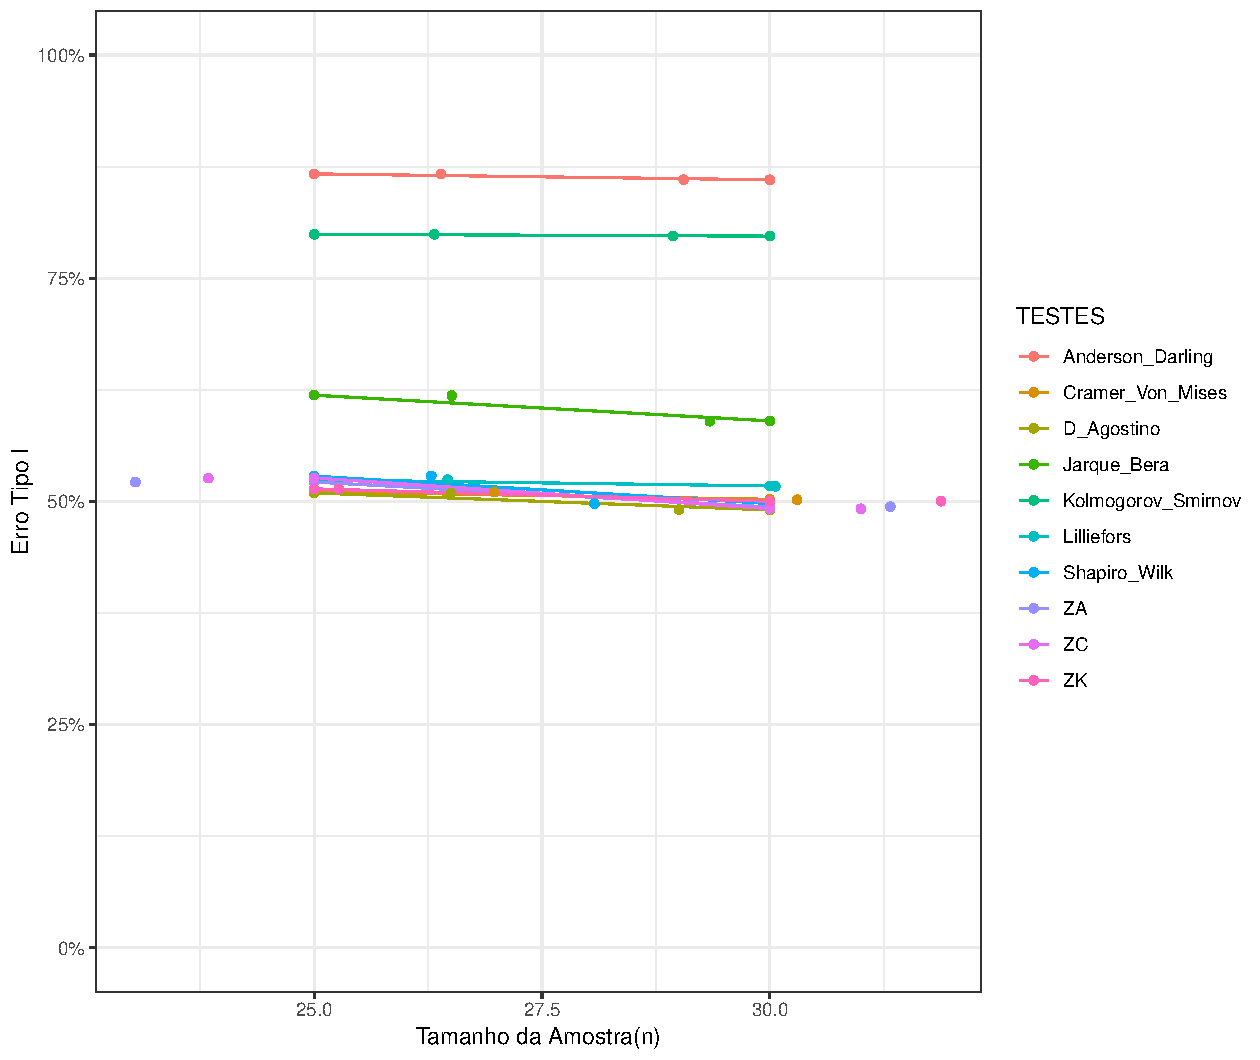
\includegraphics[width=\textwidth]{Distribuição Normal/Erro Tipo I/erro_tipo_I_normal_30.pdf}
        \caption{Tamanho amostral \(n = 30\)}
        \label{fig:normal_30}
    \end{subfigure}
    \hfill
    \begin{subfigure}[b]{0.45\textwidth}
        \centering
        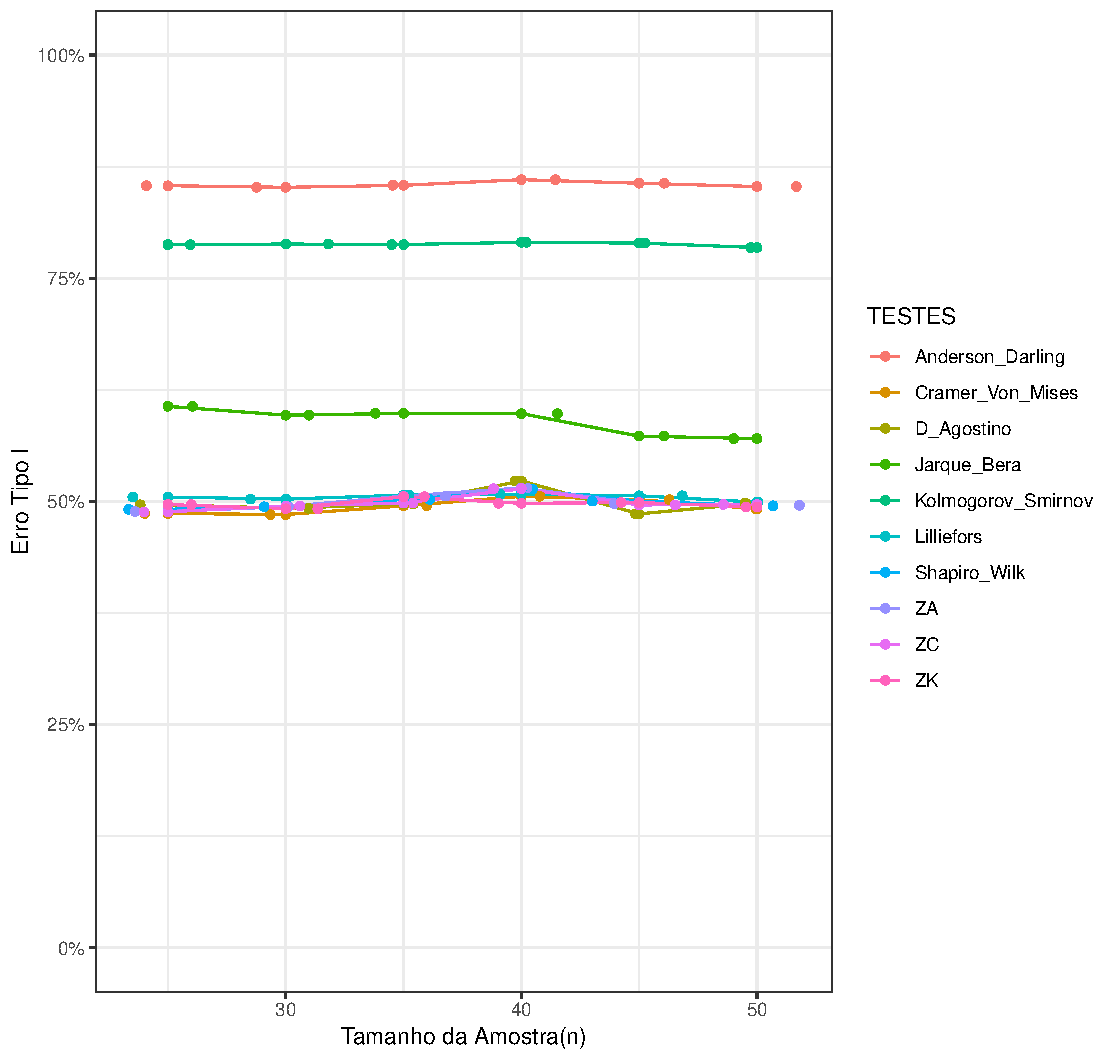
\includegraphics[width=\textwidth]{Distribuição Normal/Erro Tipo I/erro_tipo_I_normal_50.pdf}
        \caption{Tamanho amostral \(n = 50\)}
        \label{fig:normal_50}
    \end{subfigure}
    
    % Segunda linha
    \vspace{0.5cm} % Espaçamento entre linhas
    \begin{subfigure}[b]{0.45\textwidth}
        \centering
        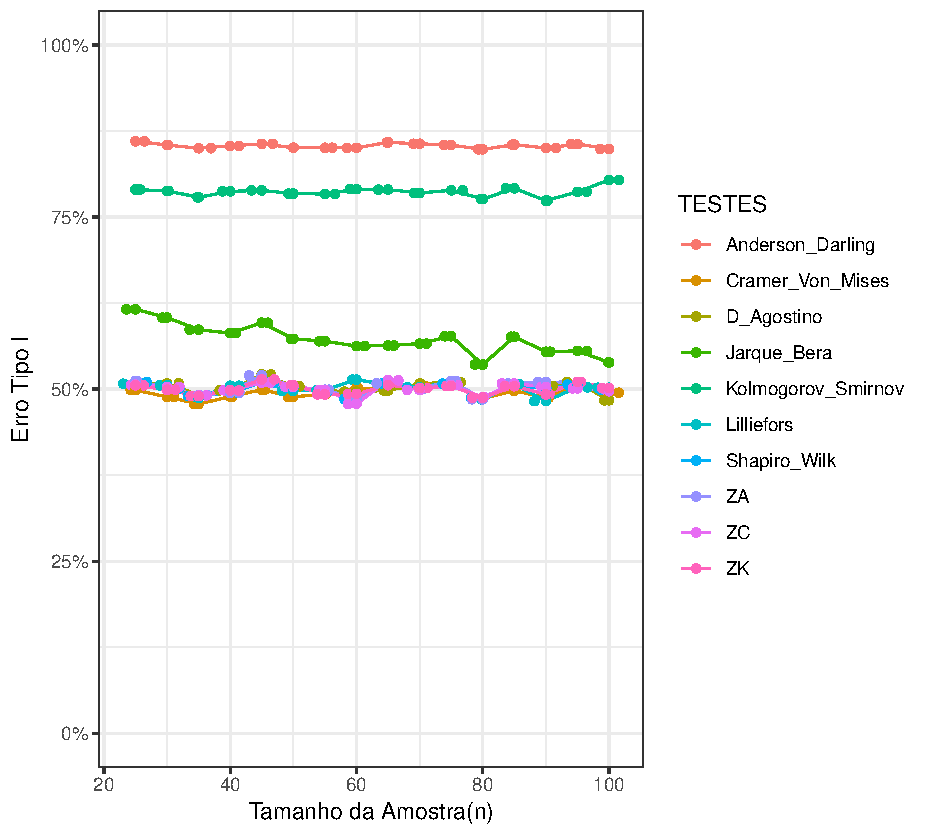
\includegraphics[width=\textwidth]{Distribuição Normal/Erro Tipo I/erro_tipo_i_normal_100.pdf}
        \caption{Tamanho amostral \(n = 100\)}
        \label{fig:normal_100}
    \end{subfigure}
    \hfill
    \begin{subfigure}[b]{0.45\textwidth}
        \centering
        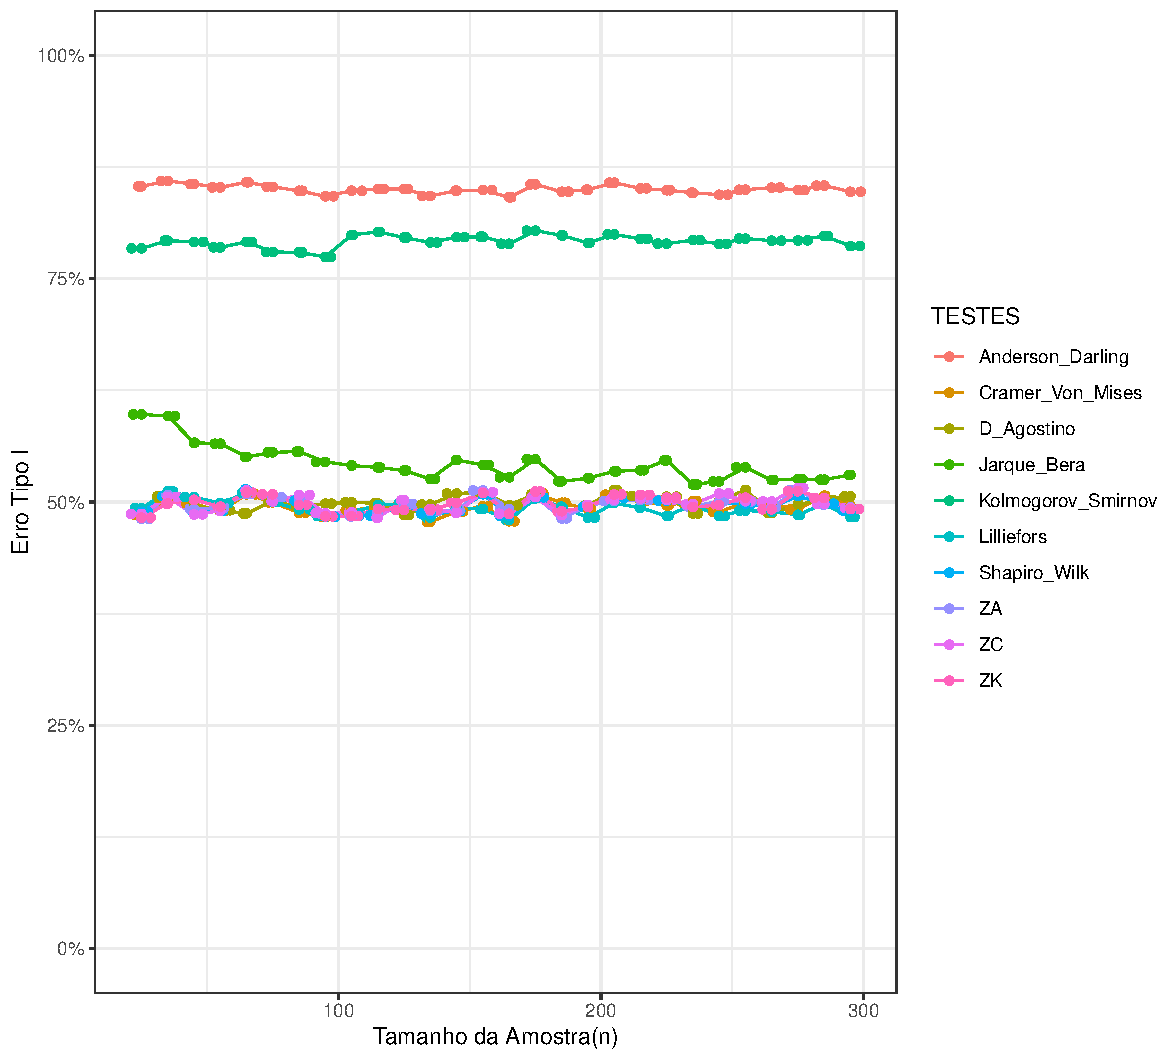
\includegraphics[width=\textwidth]{Distribuição Normal/Erro Tipo I/erro_tipo_I_normal_300.pdf}
        \caption{Tamanho amostral \(n = 300\)}
        \label{fig:normal_300}
    \end{subfigure}
    
    % Terceira linha
    \vspace{0.5cm} % Espaçamento entre linhas
    \begin{subfigure}[b]{0.45\textwidth}
        \centering
        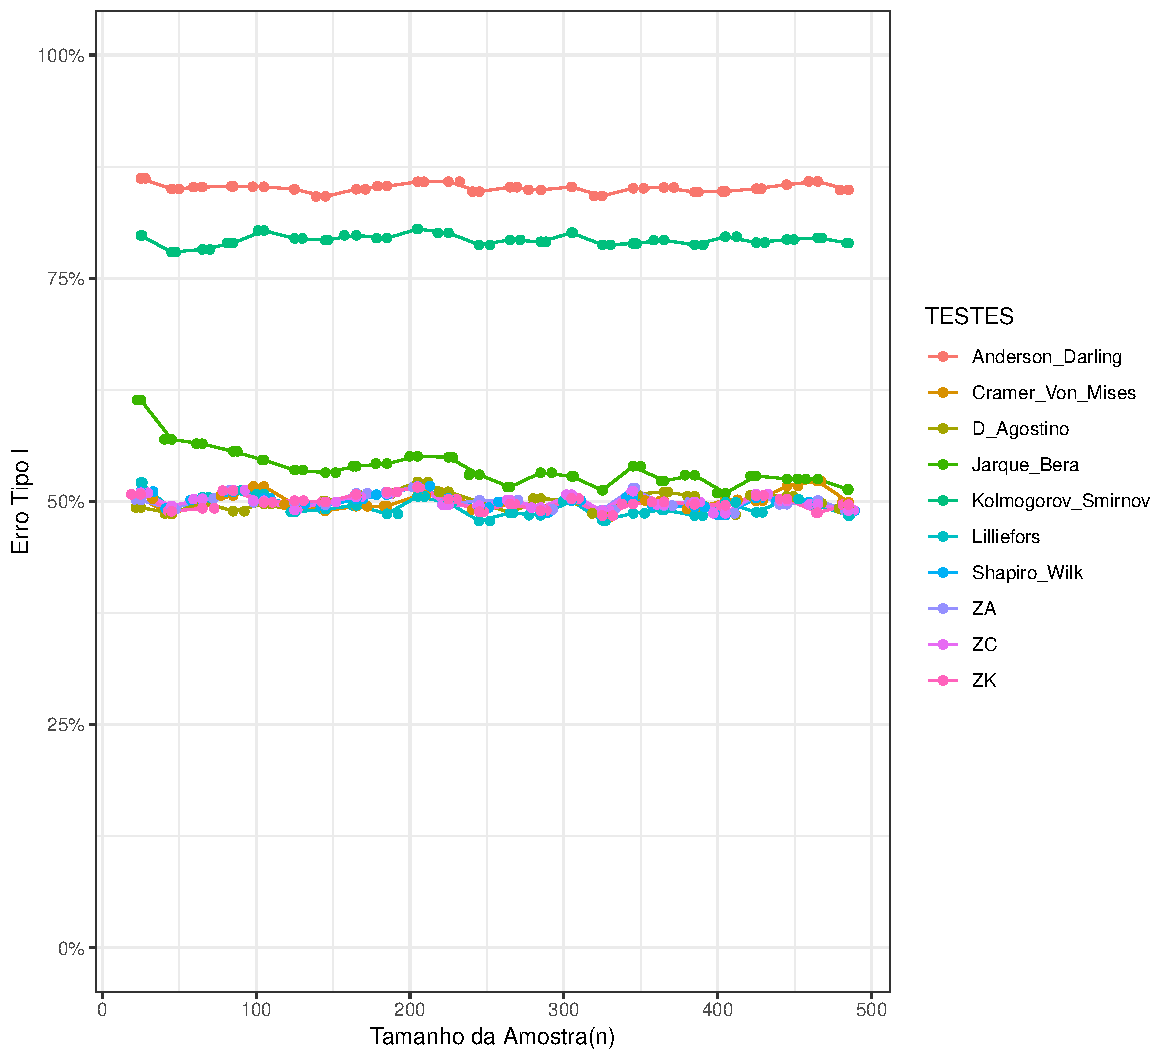
\includegraphics[width=\textwidth]{Distribuição Normal/Erro Tipo I/erro_tipo_I_normal_500.pdf}
        \caption{Tamanho amostral \(n = 500\)}
        \label{fig:normal_500}
    \end{subfigure}
    \hfill
    \begin{subfigure}[b]{0.45\textwidth}
        \centering
        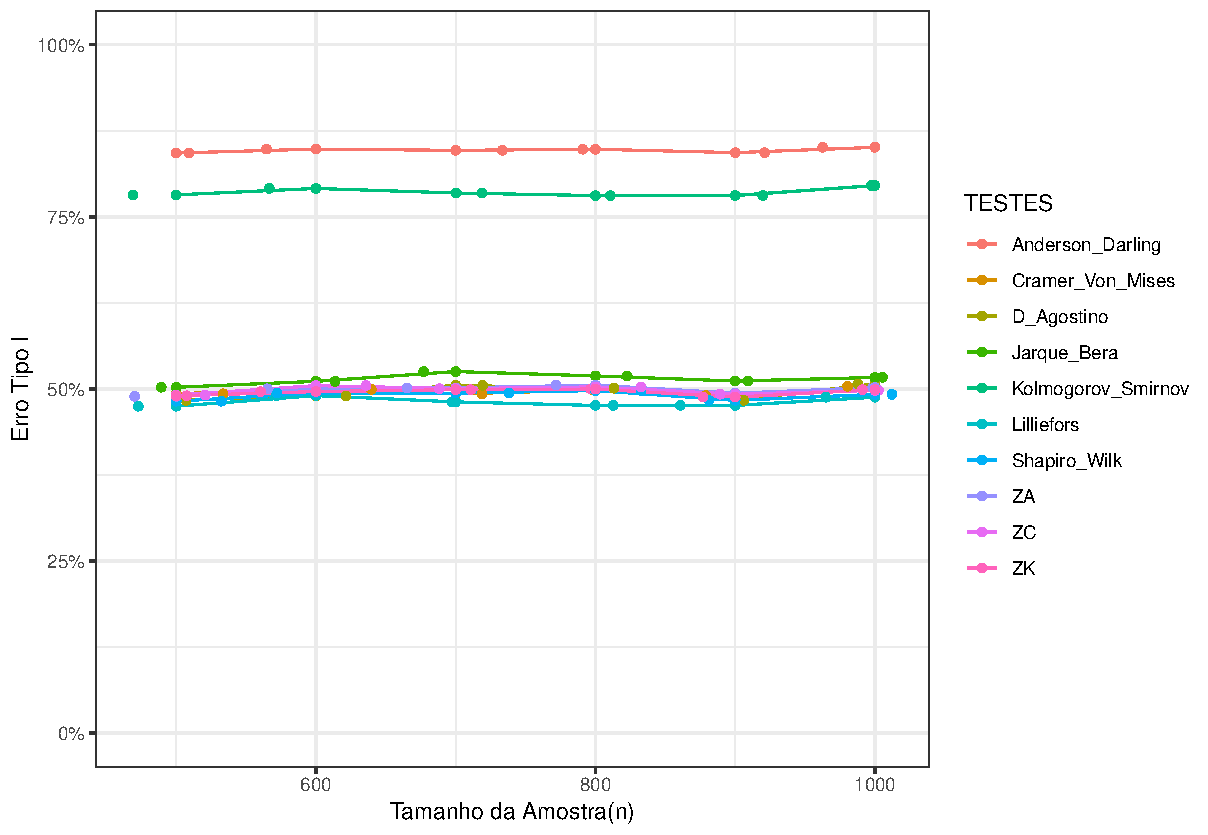
\includegraphics[width=\textwidth]{Distribuição Normal/Erro Tipo I/erro_tipo_I_normal_1000.pdf}
        \caption{Tamanho amostral \(n = 1000\)}
        \label{fig:normal_1000}
    \end{subfigure}
\end{figure}

%%%%%%%%%% Poder do Teste -> Distribuição Normal %%%%%%%%%%
\begin{figure}[H]
    \centering
    \caption{Comparação do Poder do Teste dos testes AD, CM, DG, LL, JB, KS, ZA, ZC e ZK em função do tamanho amostral para a \textbf{Distribuição} \(\textbf{Normal}(0, 1)\).}
    \label{fig:poder_teste_dist_norm}
    
    % Primeira linha
    \begin{subfigure}[b]{0.45\textwidth}
        \centering
        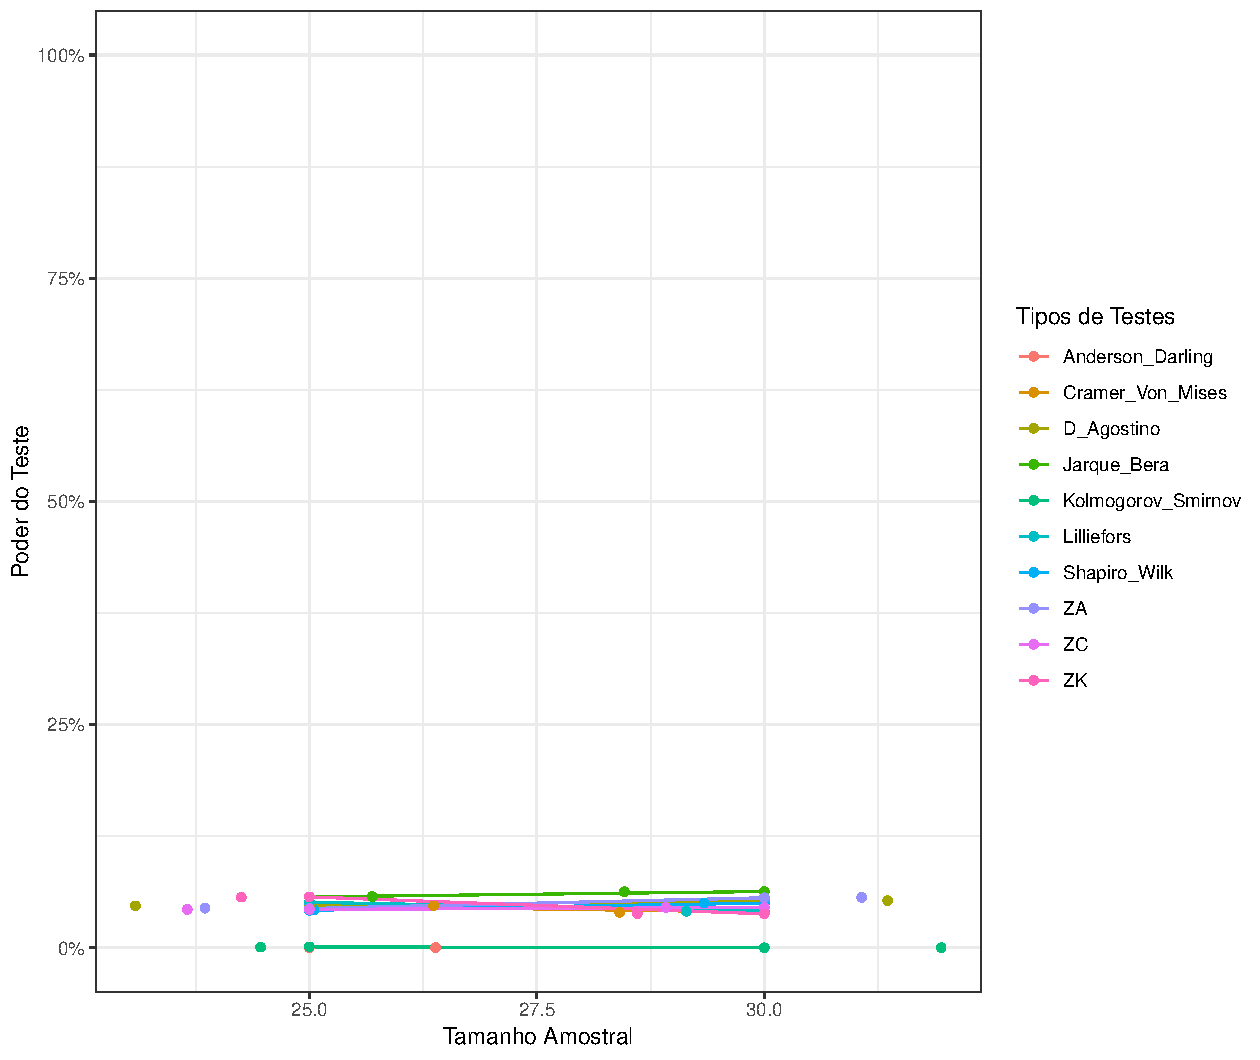
\includegraphics[width=\textwidth]{Distribuição Normal/Poder do Teste/poder_teste_normal_30.pdf}
        \caption{Tamanho amostral \(n = 30\)}
        \label{fig:normal_poder_30}
    \end{subfigure}
    \hfill
    \begin{subfigure}[b]{0.45\textwidth}
        \centering
        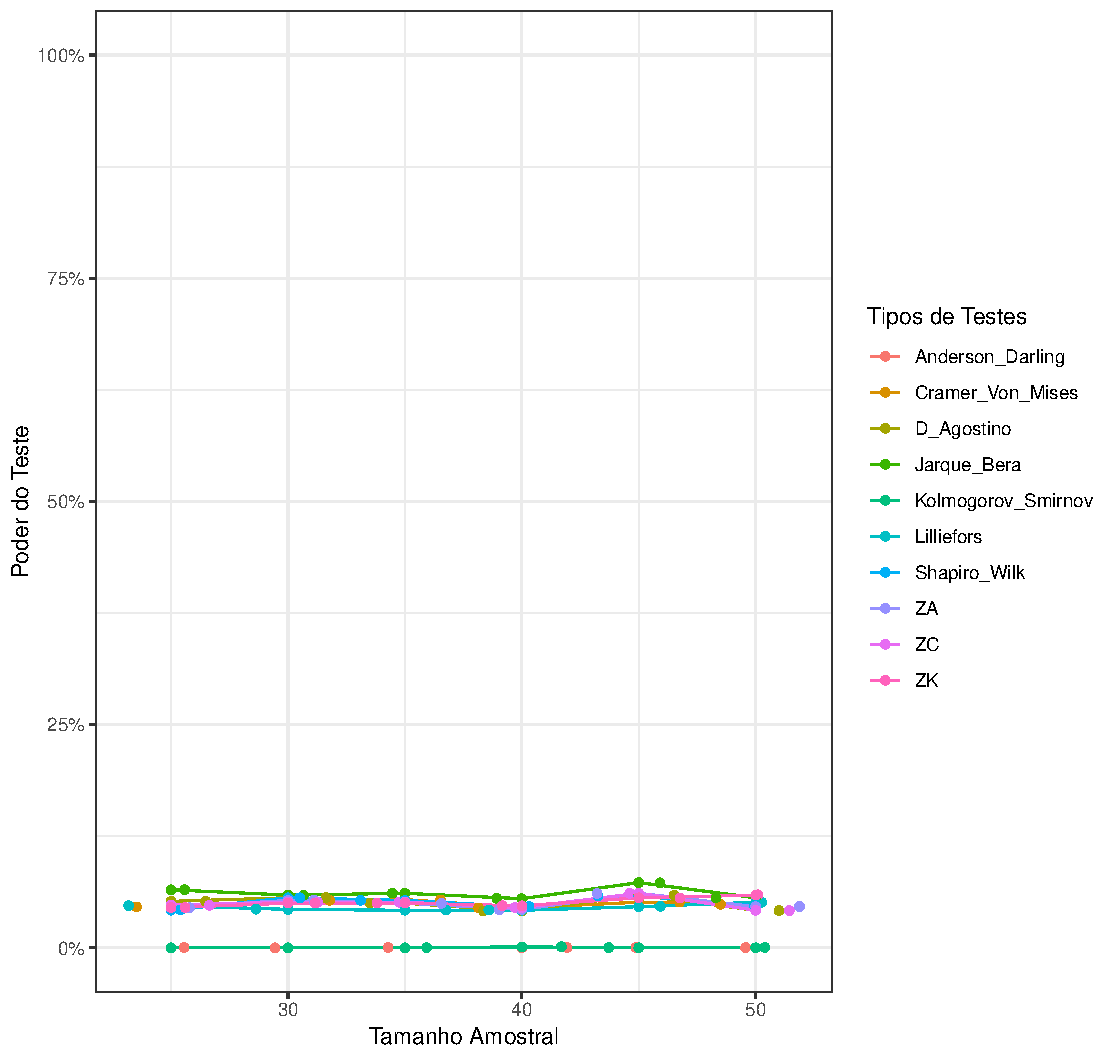
\includegraphics[width=\textwidth]{Distribuição Normal/Poder do Teste/poder_teste_normal_50.pdf}
        \caption{Tamanho amostral \(n = 50\)}
        \label{fig:normal_poder_50}
    \end{subfigure}
    
    % Segunda linha
    \vspace{0.5cm} % Espaçamento entre linhas
    \begin{subfigure}[b]{0.45\textwidth}
        \centering
        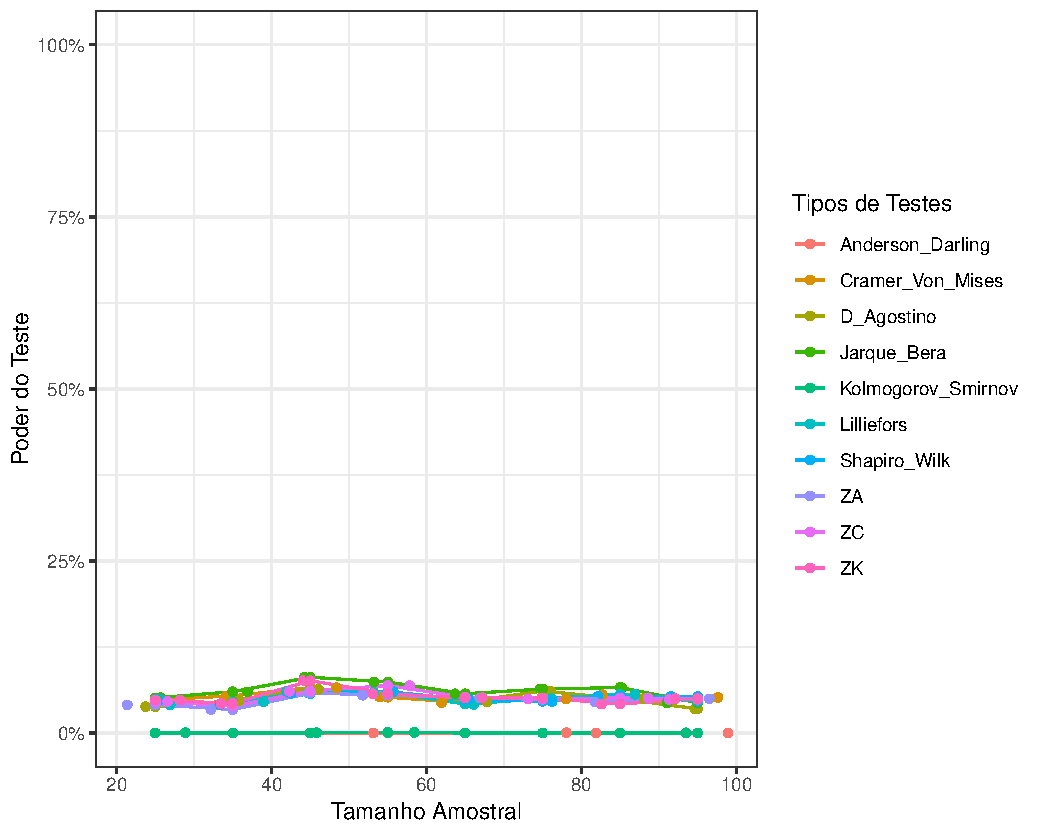
\includegraphics[width=\textwidth]{Distribuição Normal/Poder do Teste/poder_teste_normal_100.pdf}
        \caption{Tamanho amostral \(n = 100\)}
        \label{fig:normal_poder_100}
    \end{subfigure}
    \hfill
    \begin{subfigure}[b]{0.45\textwidth}
        \centering
        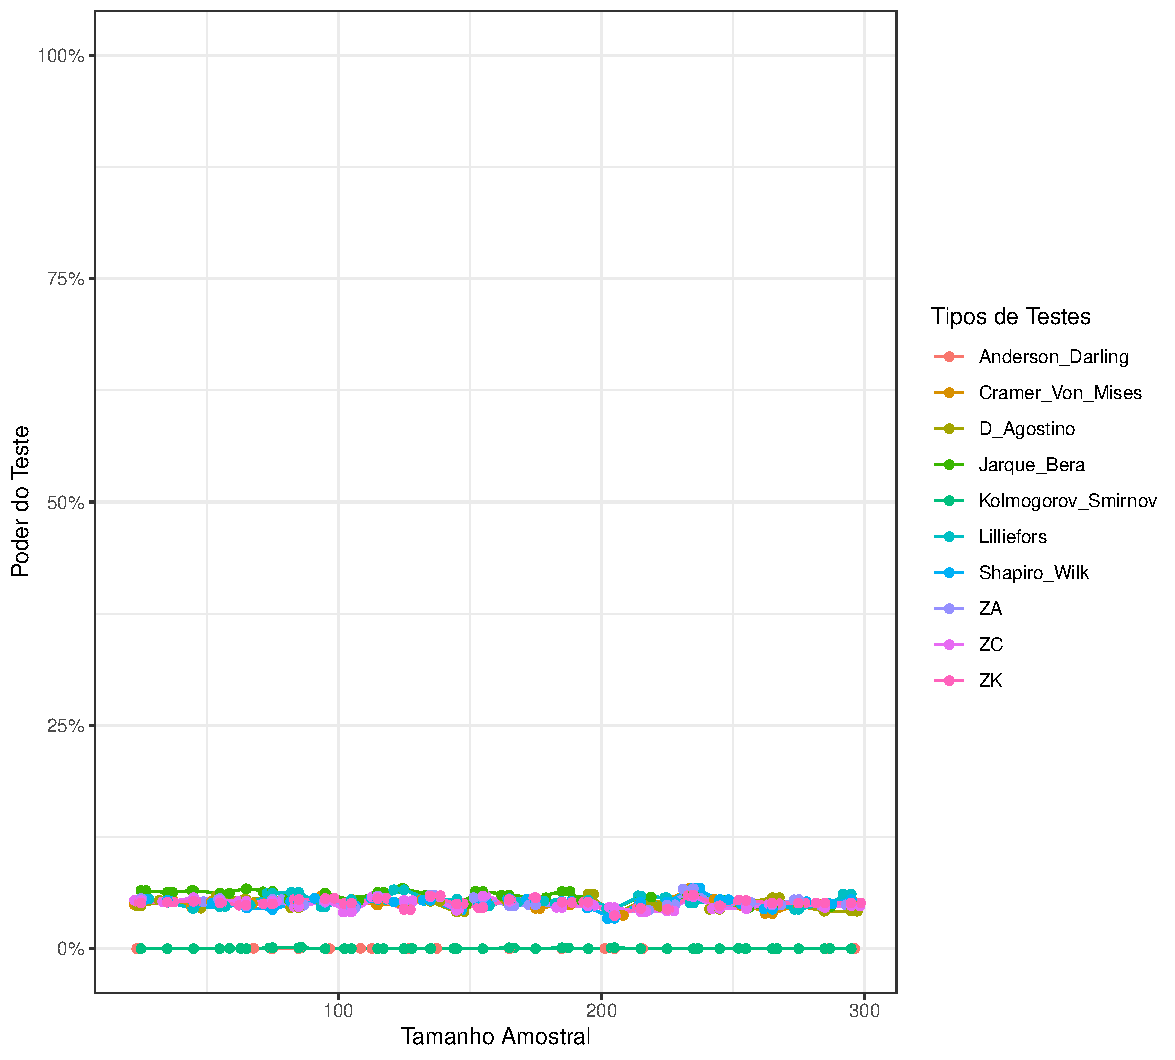
\includegraphics[width=\textwidth]{Distribuição Normal/Poder do Teste/poder_teste_normal_300.pdf}
        \caption{Tamanho amostral \(n = 300\)}
        \label{fig:normal_poder_300}
    \end{subfigure}
    
    % Terceira linha
    \vspace{0.5cm} % Espaçamento entre linhas
    \begin{subfigure}[b]{0.45\textwidth}
        \centering
        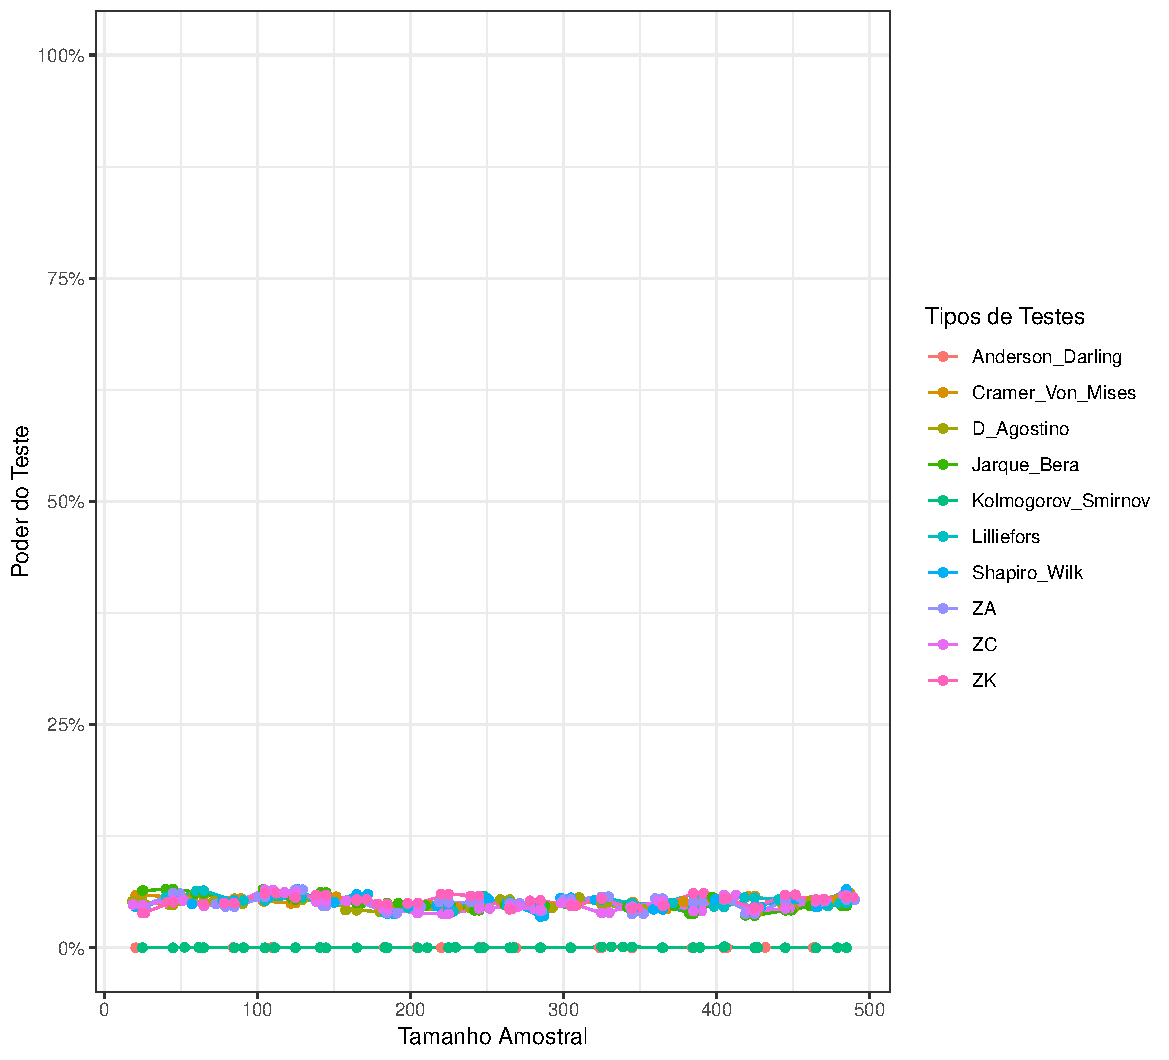
\includegraphics[width=\textwidth]{Distribuição Normal/Poder do Teste/poder_teste_normal_500.pdf}
        \caption{Tamanho amostral \(n = 500\)}
        \label{fig:normal_poder_500}
    \end{subfigure}
    \hfill
    \begin{subfigure}[b]{0.45\textwidth}
        \centering
        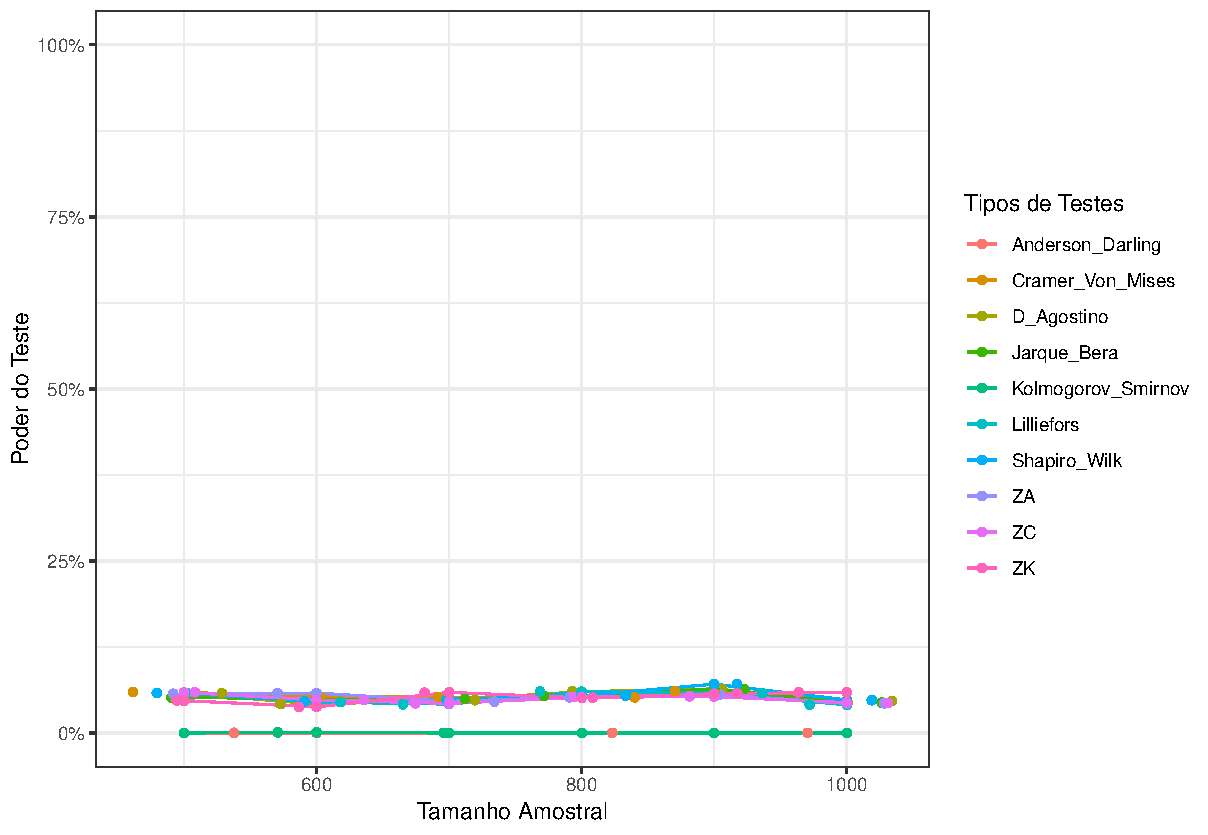
\includegraphics[width=\textwidth]{Distribuição Normal/Poder do Teste/poder_teste_normal_1000.pdf}
        \caption{Tamanho amostral \(n = 1000\)}
        \label{fig:normal_poder_1000}
    \end{subfigure}
\end{figure}

%%%%%%%%%% Erro Tipo I -> Distribuição Beta %%%%%%%%%%
\begin{figure}[H]
    \centering
    \caption{Comparação do Erro Tipo I dos testes AD, CM, DG, LL, JB, KS, LL, ZA, ZC e ZK em função do tamanho amostral para a \textbf{Distribuição} $\textbf{Beta}(2, 5)$.}
    \label{fig:erro_tipo_I_dist_beta}
    
    % Primeira linha
    \begin{subfigure}[b]{0.45\textwidth}
        \centering
        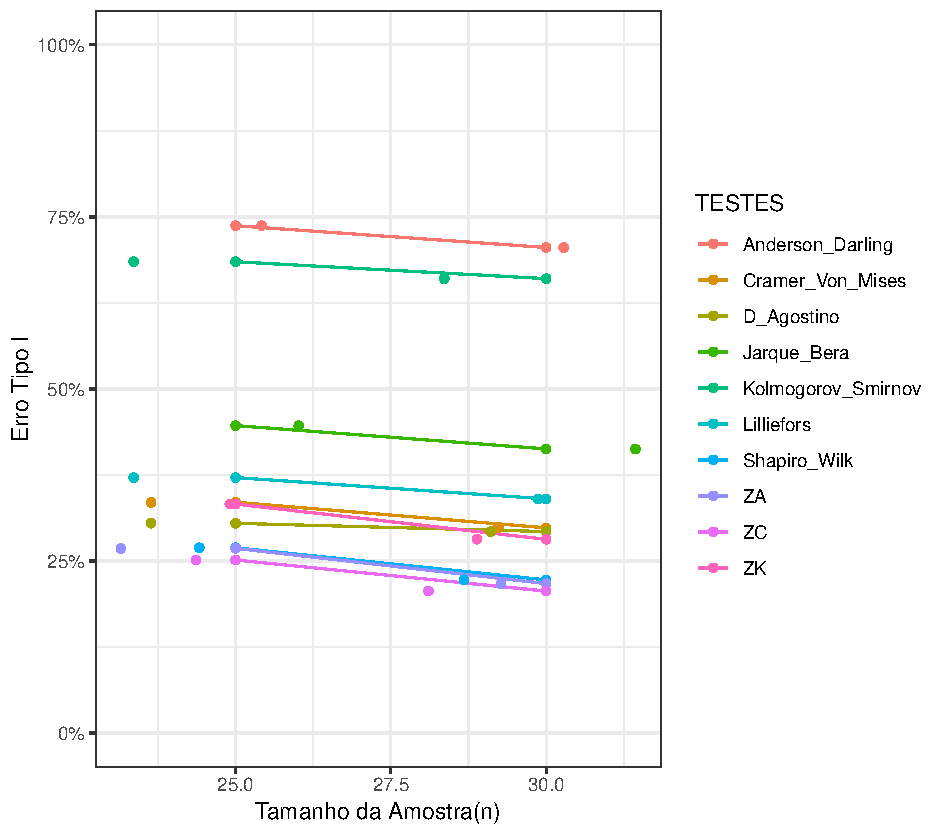
\includegraphics[width=\textwidth]{Distribuição Beta/Erro Tipo I/erro_tipo_I_beta_30.pdf}
        \caption{Tamanho amostral \(n = 30\)}
        \label{fig:beta_30}
    \end{subfigure}
    \hfill
    \begin{subfigure}[b]{0.45\textwidth}
        \centering
        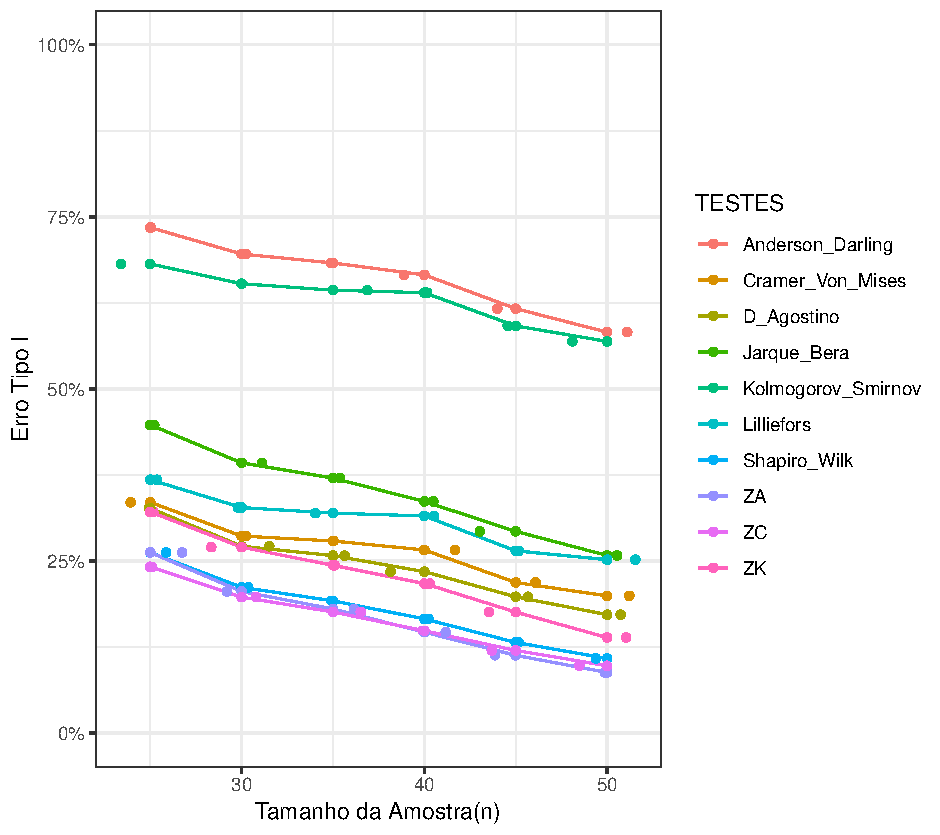
\includegraphics[width=\textwidth]{Distribuição Beta/Erro Tipo I/erro_tipo_I_beta_50.pdf}
        \caption{Tamanho amostral \(n = 50\)}
        \label{fig:beta_50}
    \end{subfigure}
    
    % Segunda linha
    \vspace{0.5cm} % Espaçamento entre linhas
    \begin{subfigure}[b]{0.45\textwidth}
        \centering
        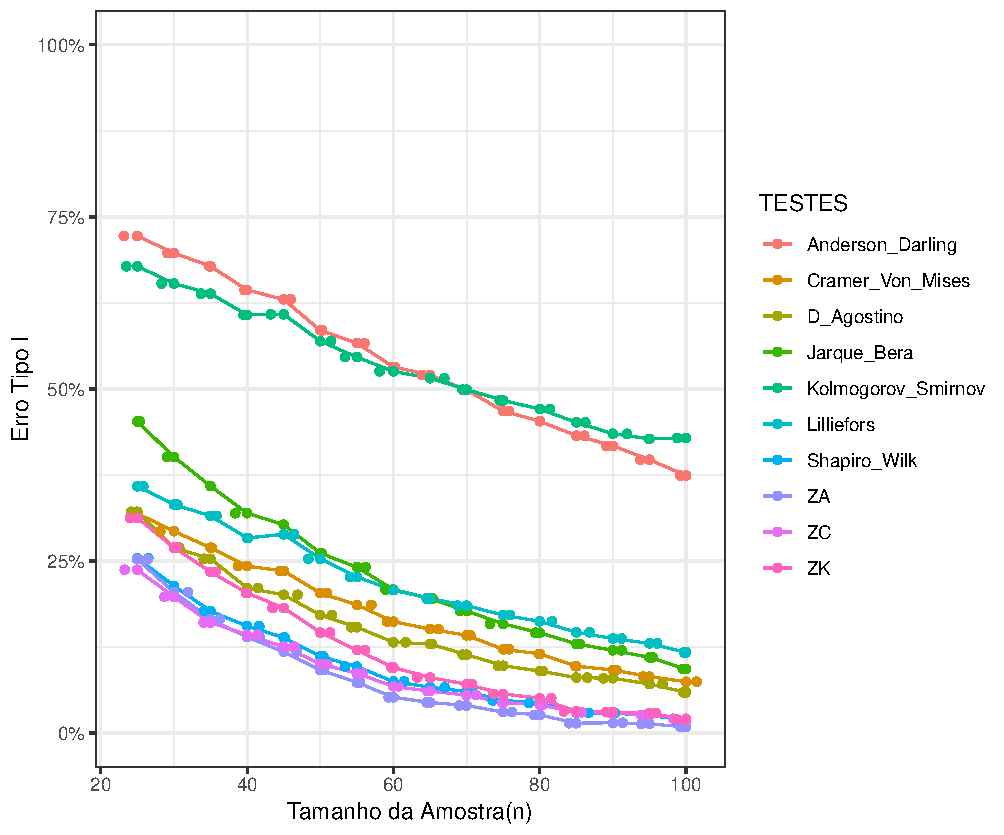
\includegraphics[width=\textwidth]{Distribuição Beta/Erro Tipo I/erro_tipo_I_beta_100.pdf}
        \caption{Tamanho amostral \(n = 100\)}
        \label{fig:beta_100}
    \end{subfigure}
    \hfill
    \begin{subfigure}[b]{0.45\textwidth}
        \centering
        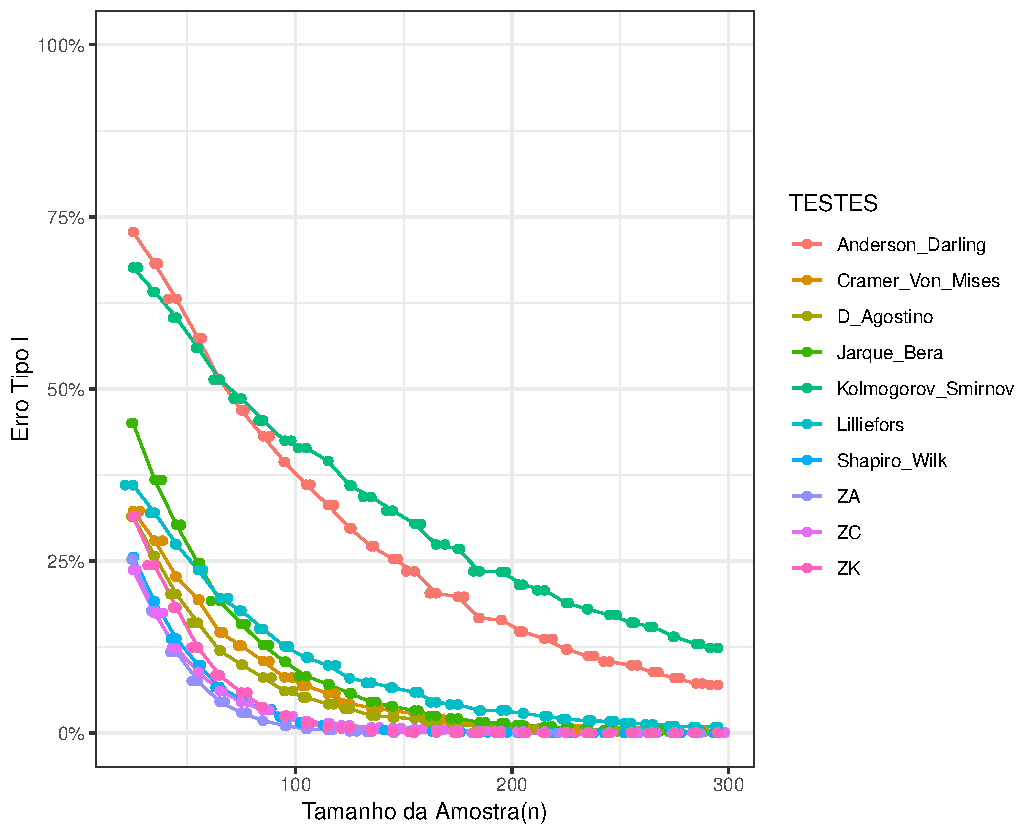
\includegraphics[width=\textwidth]{Distribuição Beta/Erro Tipo I/erro_tipo_I_beta_300.pdf}
        \caption{Tamanho amostral \(n = 300\)}
        \label{fig:beta_300}
    \end{subfigure}
    
    % Terceira linha
    \vspace{0.5cm} % Espaçamento entre linhas
    \begin{subfigure}[b]{0.45\textwidth}
        \centering
        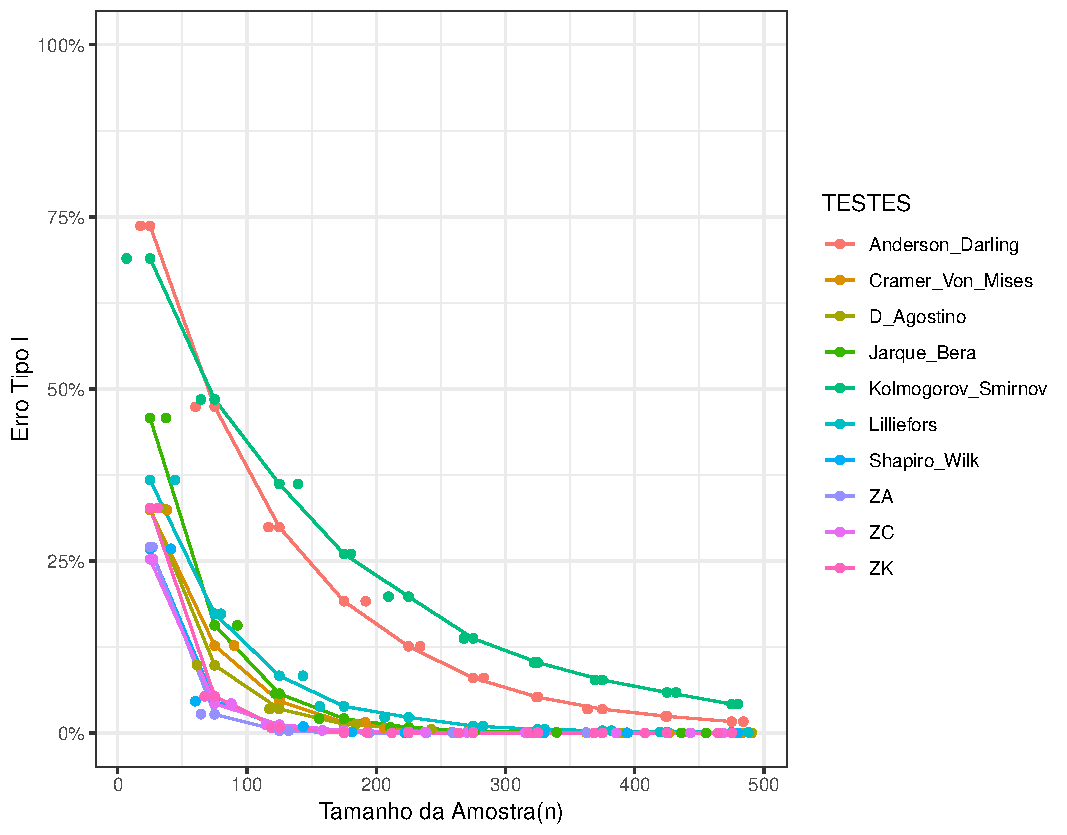
\includegraphics[width=\textwidth]{Distribuição Beta/Erro Tipo I/erro_tipo_I_beta_500.pdf}
        \caption{Tamanho amostral \(n = 500\)}
        \label{fig:beta_500}
    \end{subfigure}
    \hfill
    \begin{subfigure}[b]{0.45\textwidth}
        \centering
        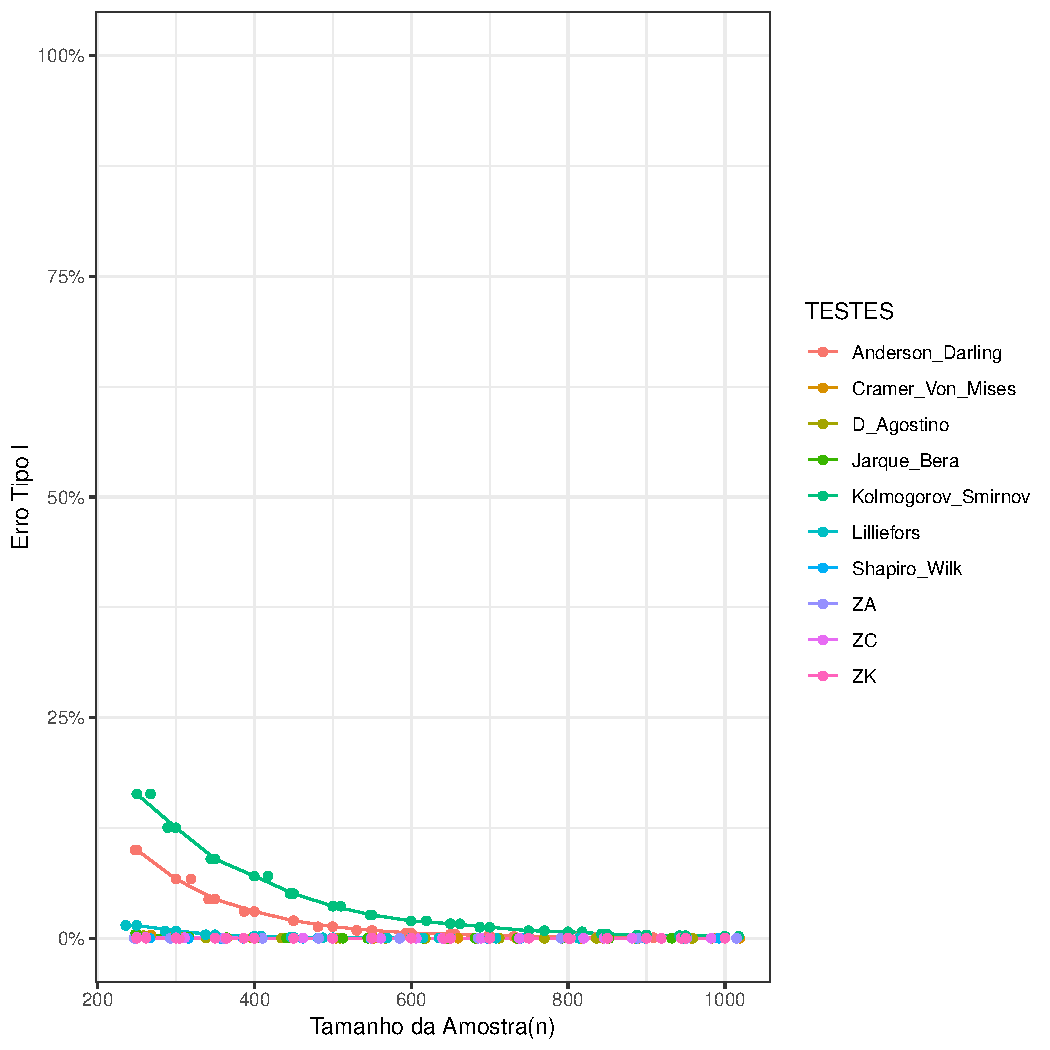
\includegraphics[width=\textwidth]{Distribuição Beta/Erro Tipo I/erro_tipo_I_beta_1000.pdf}
        \caption{Tamanho amostral \(n = 1000\)}
        \label{fig:beta_1000}
    \end{subfigure}
\end{figure}

%%%%%%%%%% Poder do Teste -> Distribuição Beta %%%%%%%%%%
\begin{figure}[H]
    \centering
    \caption{Comparação do Poder do Teste dos testes AD, CM, DG, LL, JB, KS, ZA, ZC e ZK em função do tamanho amostral para a \textbf{Distribuição} \(\textbf{Beta}(2, 5)\).}
    \label{fig:poder_teste_dist_beta}
    
    % Primeira linha
    \begin{subfigure}[b]{0.45\textwidth}
        \centering
        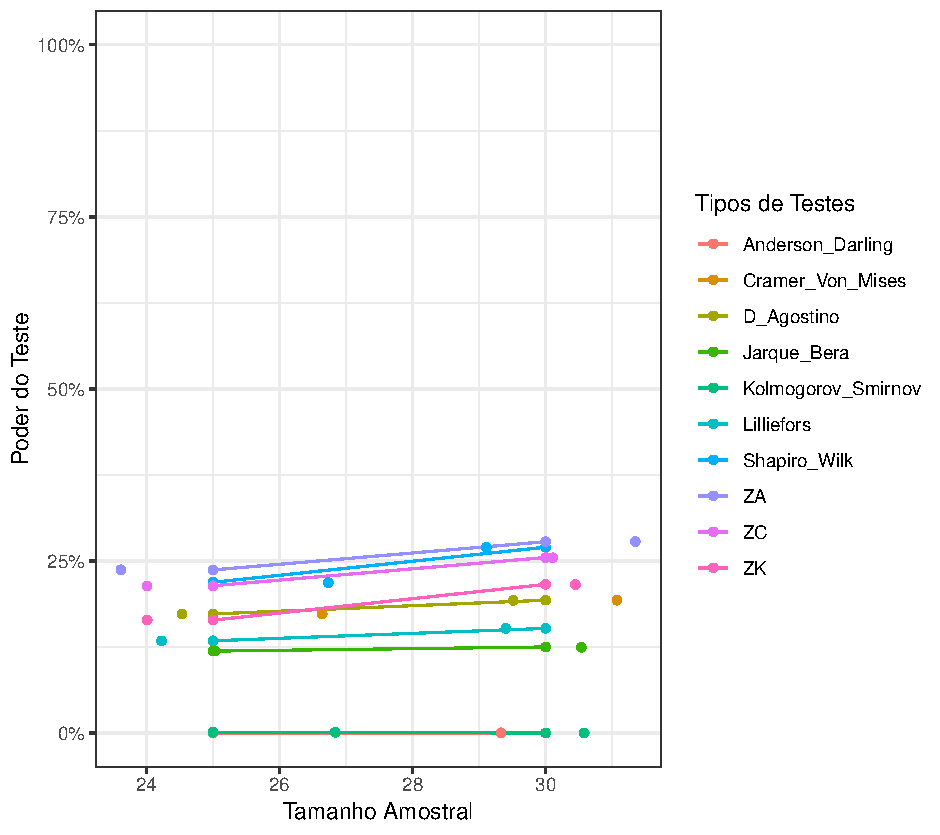
\includegraphics[width=\textwidth]{Distribuição Beta/Poder do Teste/poder_teste_beta_30.pdf}
        \caption{Tamanho amostral \(n = 30\)}
        \label{fig:beta_poder_30}
    \end{subfigure}
    \hfill
    \begin{subfigure}[b]{0.45\textwidth}
        \centering
        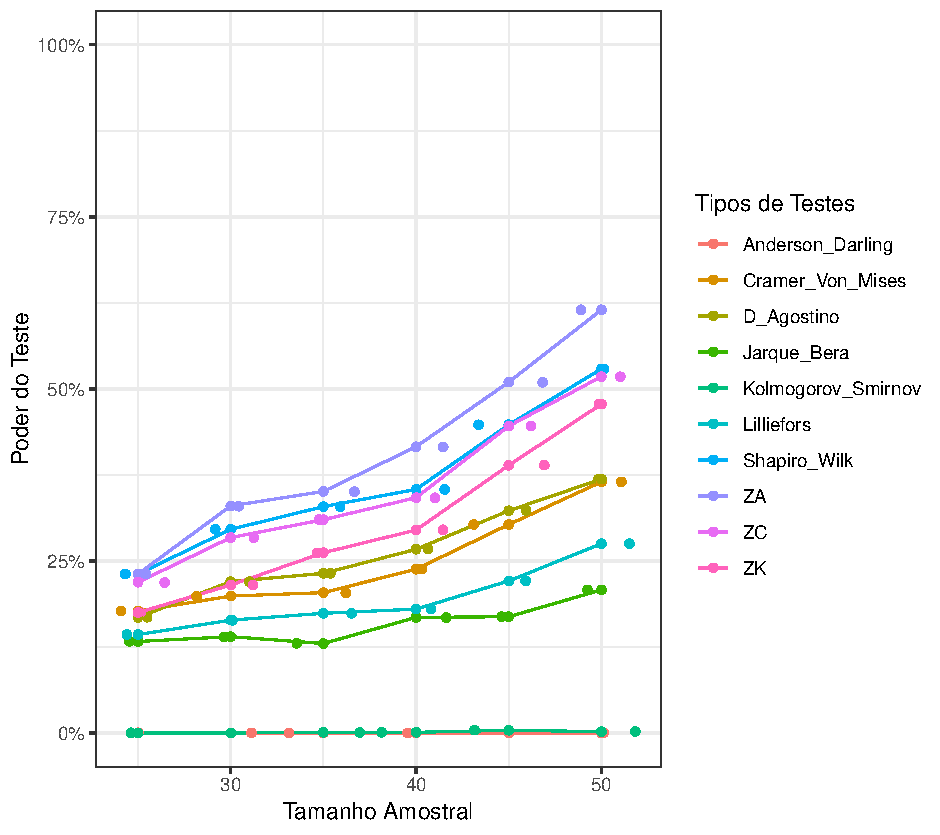
\includegraphics[width=\textwidth]{Distribuição Beta/Poder do Teste/poder_teste_beta_50.pdf}
        \caption{Tamanho amostral \(n = 50\)}
        \label{fig:beta_poder_50}
    \end{subfigure}
    
    % Segunda linha
    \vspace{0.5cm} % Espaçamento entre linhas
    \begin{subfigure}[b]{0.45\textwidth}
        \centering
        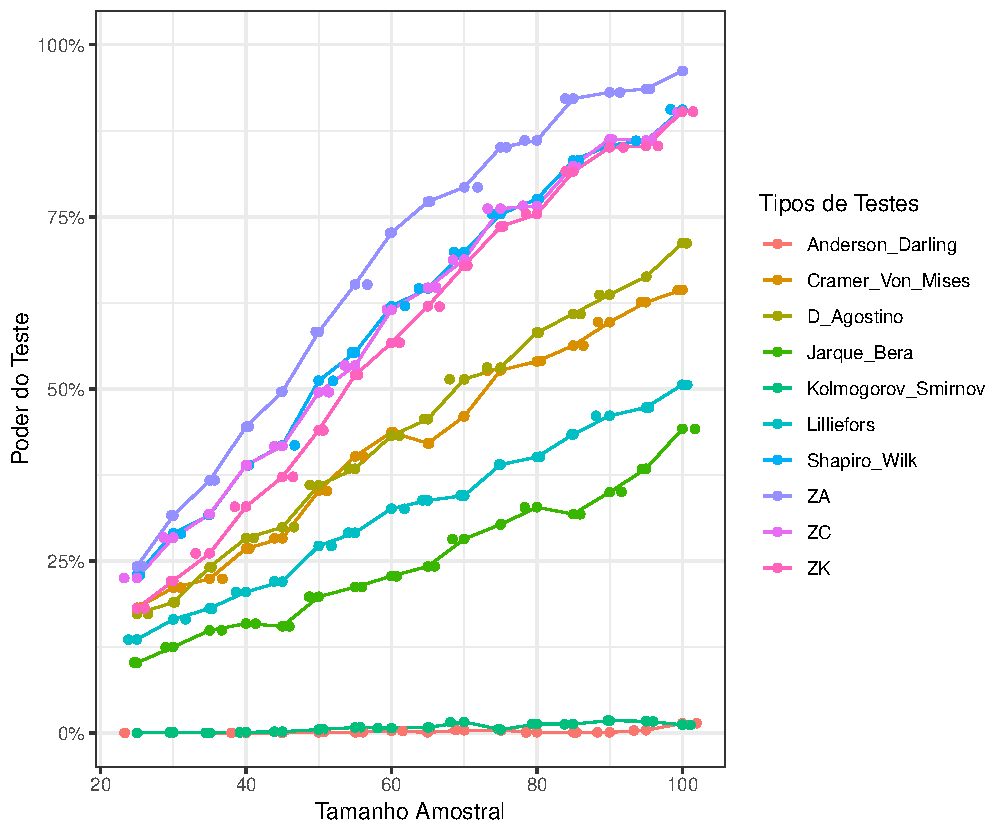
\includegraphics[width=\textwidth]{Distribuição Beta/Poder do Teste/poder_teste_beta_100.pdf}
        \caption{Tamanho amostral \(n = 100\)}
        \label{fig:beta_poder_100}
    \end{subfigure}
    \hfill
    \begin{subfigure}[b]{0.45\textwidth}
        \centering
        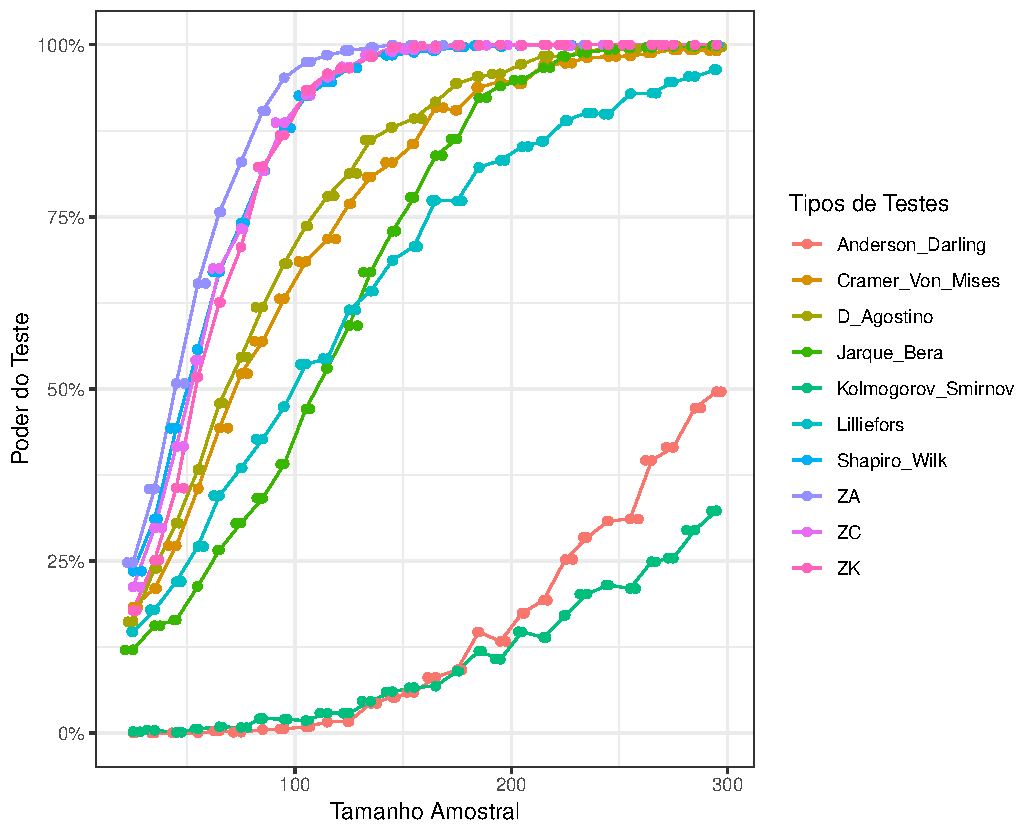
\includegraphics[width=\textwidth]{Distribuição Beta/Poder do Teste/poder_teste_beta_300.pdf}
        \caption{Tamanho amostral \(n = 300\)}
        \label{fig:beta_poder_300}
    \end{subfigure}
    
    % Terceira linha
    \vspace{0.5cm} % Espaçamento entre linhas
    \begin{subfigure}[b]{0.45\textwidth}
        \centering
        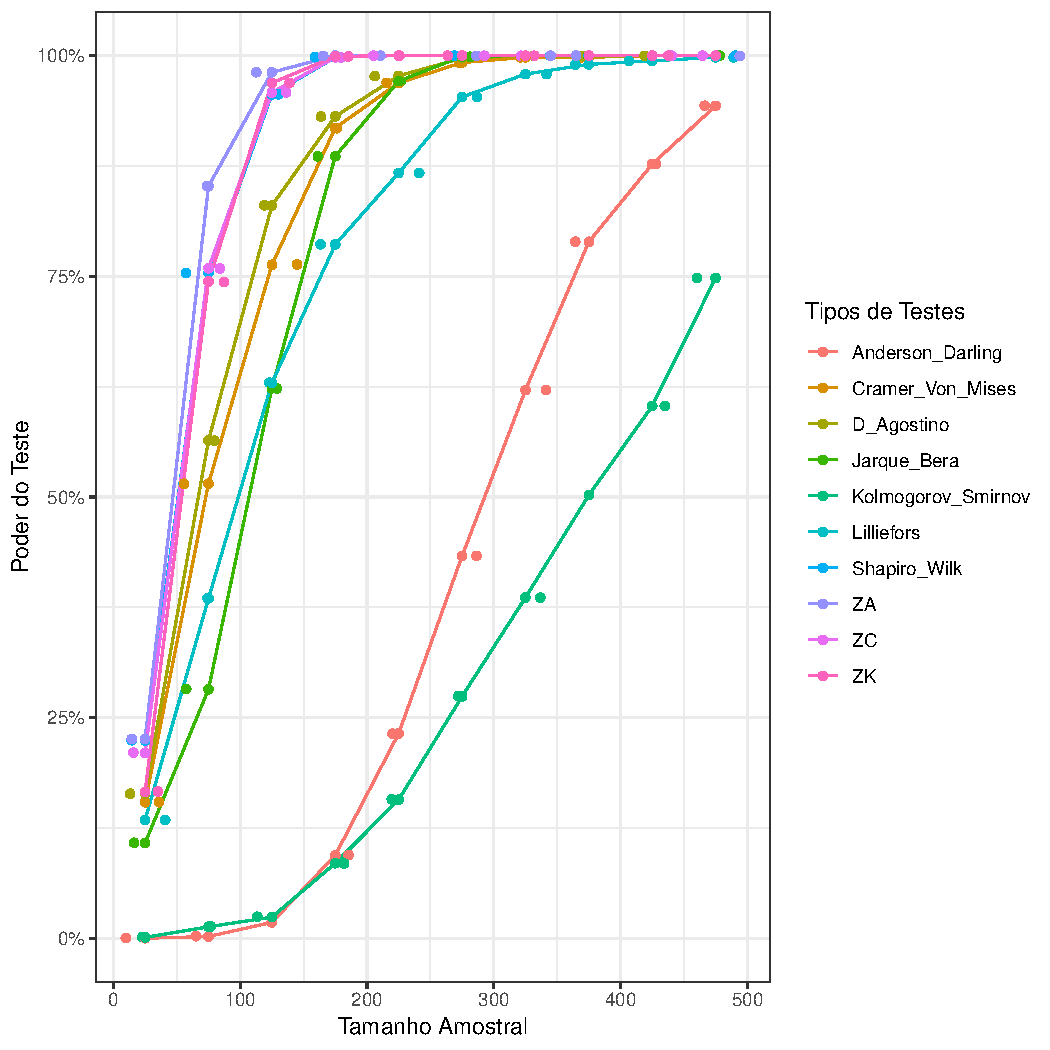
\includegraphics[width=\textwidth]{Distribuição Beta/Poder do Teste/poder_teste_beta_500.pdf}
        \caption{Tamanho amostral \(n = 500\)}
        \label{fig:beta_poder_500}
    \end{subfigure}
    \hfill
    \begin{subfigure}[b]{0.45\textwidth}
        \centering
        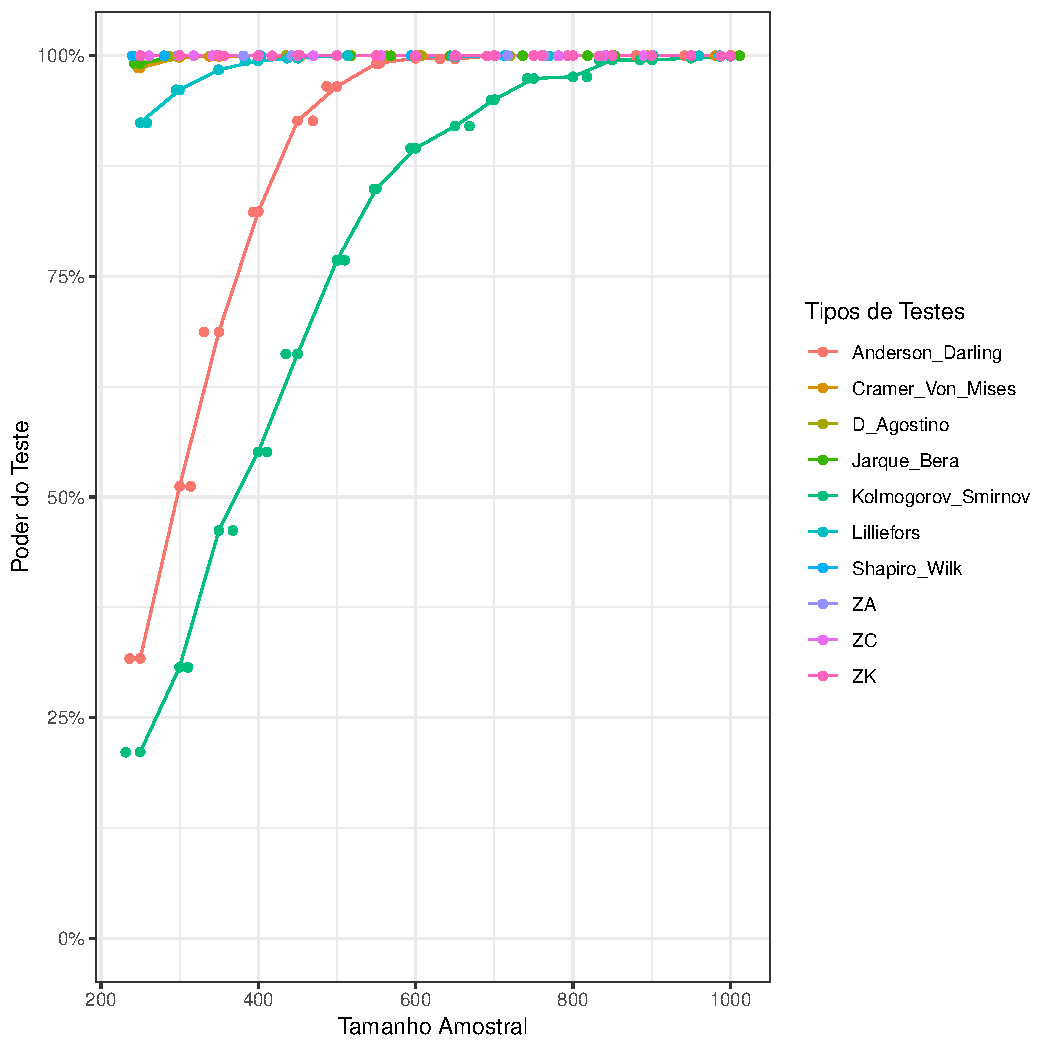
\includegraphics[width=\textwidth]{Distribuição Beta/Poder do Teste/poder_teste_beta_1000.pdf}
        \caption{Tamanho amostral \(n = 1000\)}
        \label{fig:beta_poder_1000}
    \end{subfigure}
\end{figure}


%%%%%%%%%%%%%%%%%%%%%%%%%%%%%%%%%%%%%%%%%%%%%%%%%%%%%%%%%%%%%%%%%%%%%%%%%%%%%%%%%%%%%%%%%%%%

%%%%%%%%%% Erro Tipo I -> Distribuição Cauchy %%%%%%%%%%
\begin{figure}[H]
    \centering
    \caption{Comparação do Erro Tipo I dos testes AD, CM, DG, LL, JB, KS, LL, ZA, ZC e ZK em função do tamanho amostral para a \textbf{Distribuição} $\textbf{Cauchy}(0, 1)$.}
    \label{fig:erro_tipo_I_dist_cauchy}
    
    % Primeira linha
    \begin{subfigure}[b]{0.45\textwidth}
        \centering
    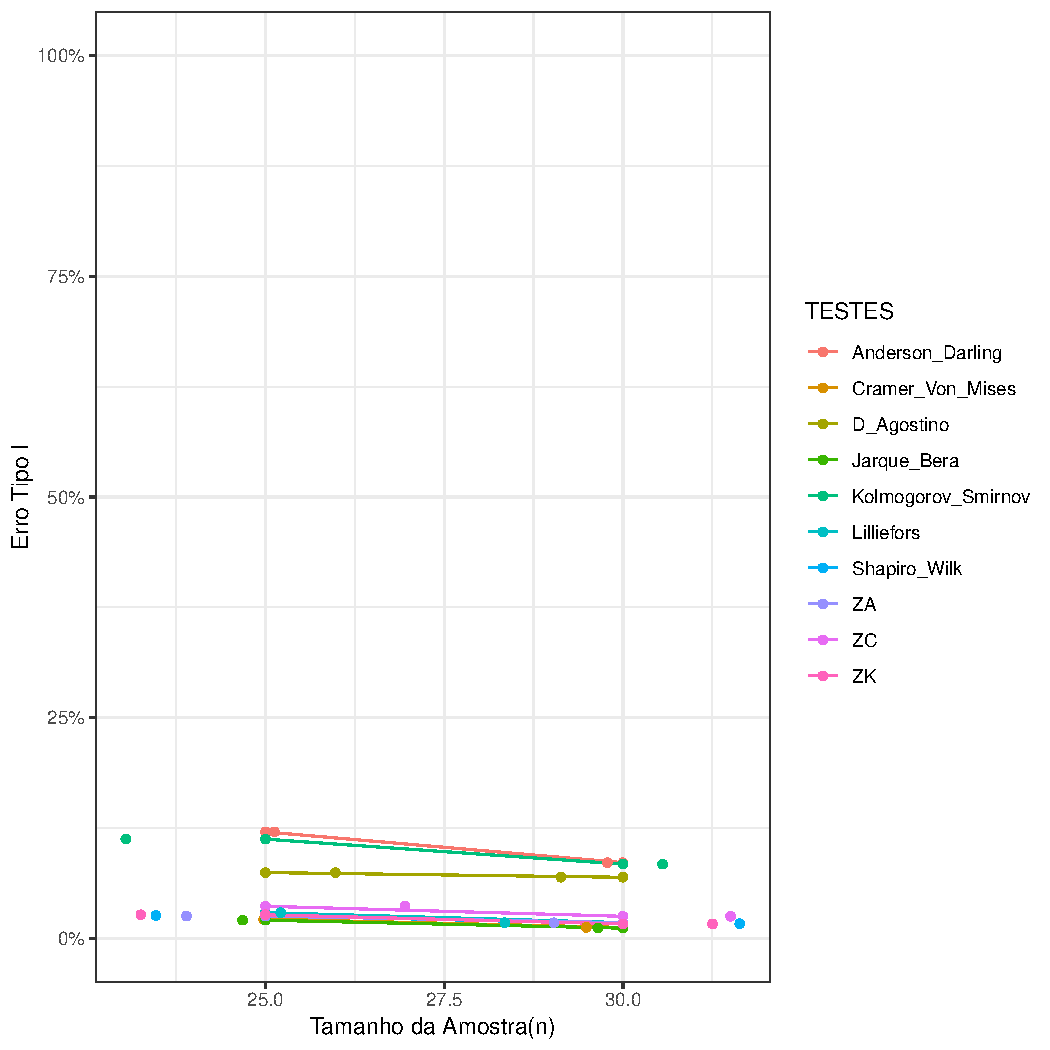
\includegraphics[width=0.95\textwidth]{Distribuição Cauchy/Erro Tipo I/erro_tipo_I_cauchy_30.pdf}
        \caption{Tamanho amostral \(n = 30\)}
        \label{fig:cauchy_30}
    \end{subfigure}
    \hfill
    \begin{subfigure}[b]{0.45\textwidth}
        \centering
        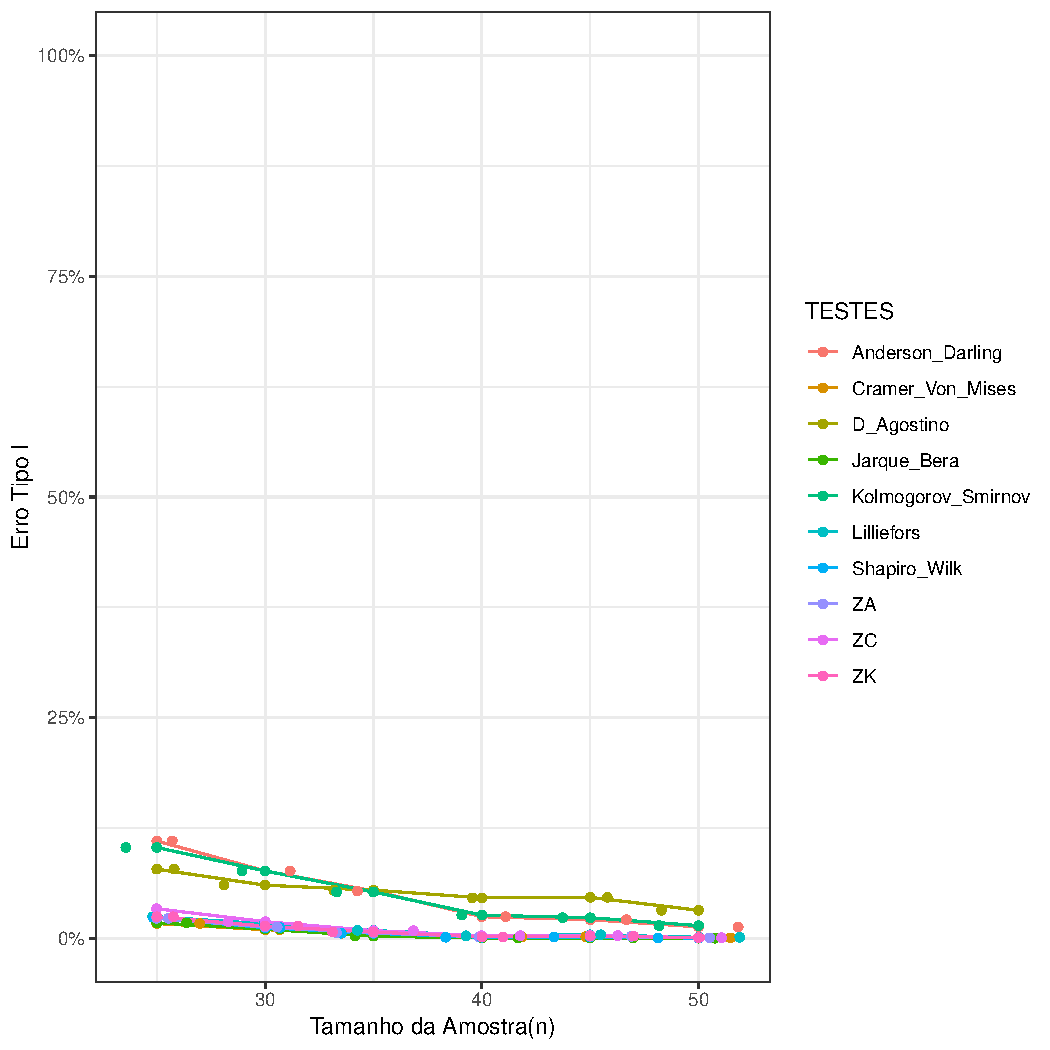
\includegraphics[width=0.95\textwidth]{Distribuição Cauchy/Erro Tipo I/erro_tipo_I_cauchy_50.pdf}
        \caption{Tamanho amostral \(n = 50\)}
        \label{fig:cauchy_50}
    \end{subfigure}
    
    % Segunda linha
    \vspace{0.5cm} % Espaçamento entre linhas
    \begin{subfigure}[b]{0.45\textwidth}
        \centering
        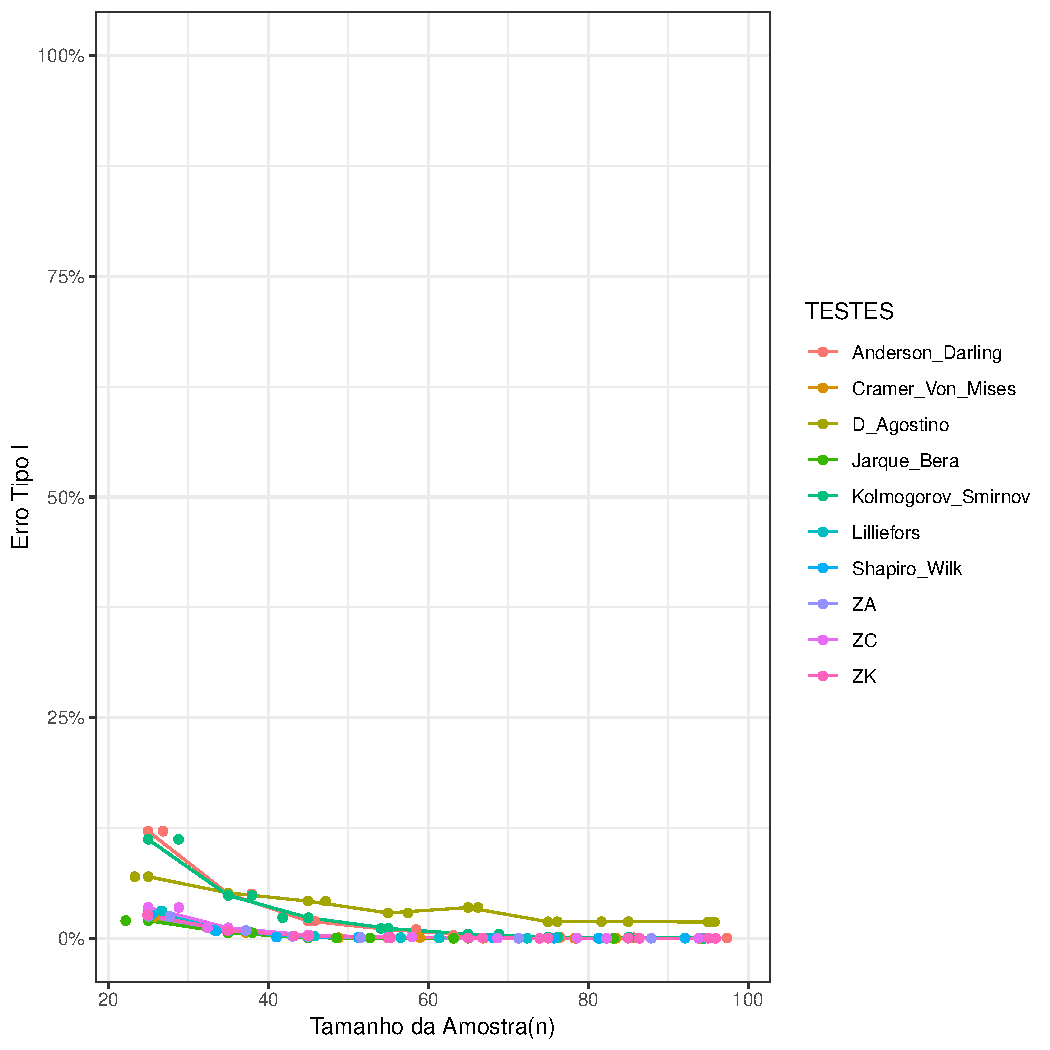
\includegraphics[width=0.95\textwidth]{Distribuição Cauchy/Erro Tipo I/erro_tipo_I_cauchy_100.pdf}
        \caption{Tamanho amostral \(n = 100\)}
        \label{fig:cauchy_100}
    \end{subfigure}
    \hfill
    \begin{subfigure}[b]{0.45\textwidth}
        \centering
        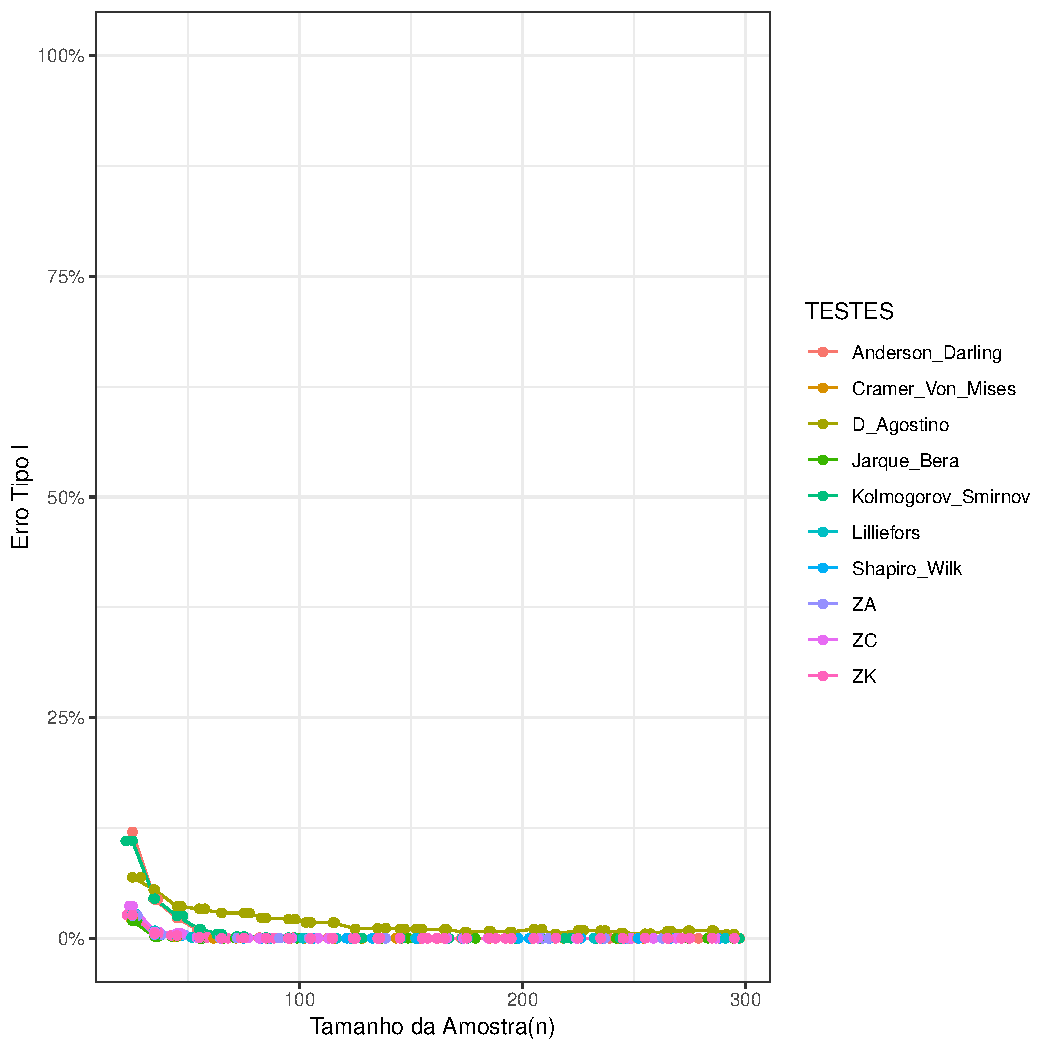
\includegraphics[width=0.95\textwidth]{Distribuição Cauchy/Erro Tipo I/erro_tipo_I_cauchy_300.pdf}
        \caption{Tamanho amostral \(n = 300\)}
        \label{fig:cauchy_300}
    \end{subfigure}
    
    % Terceira linha
    \vspace{0.5cm} % Espaçamento entre linhas
    \begin{subfigure}[b]{0.45\textwidth}
        \centering
        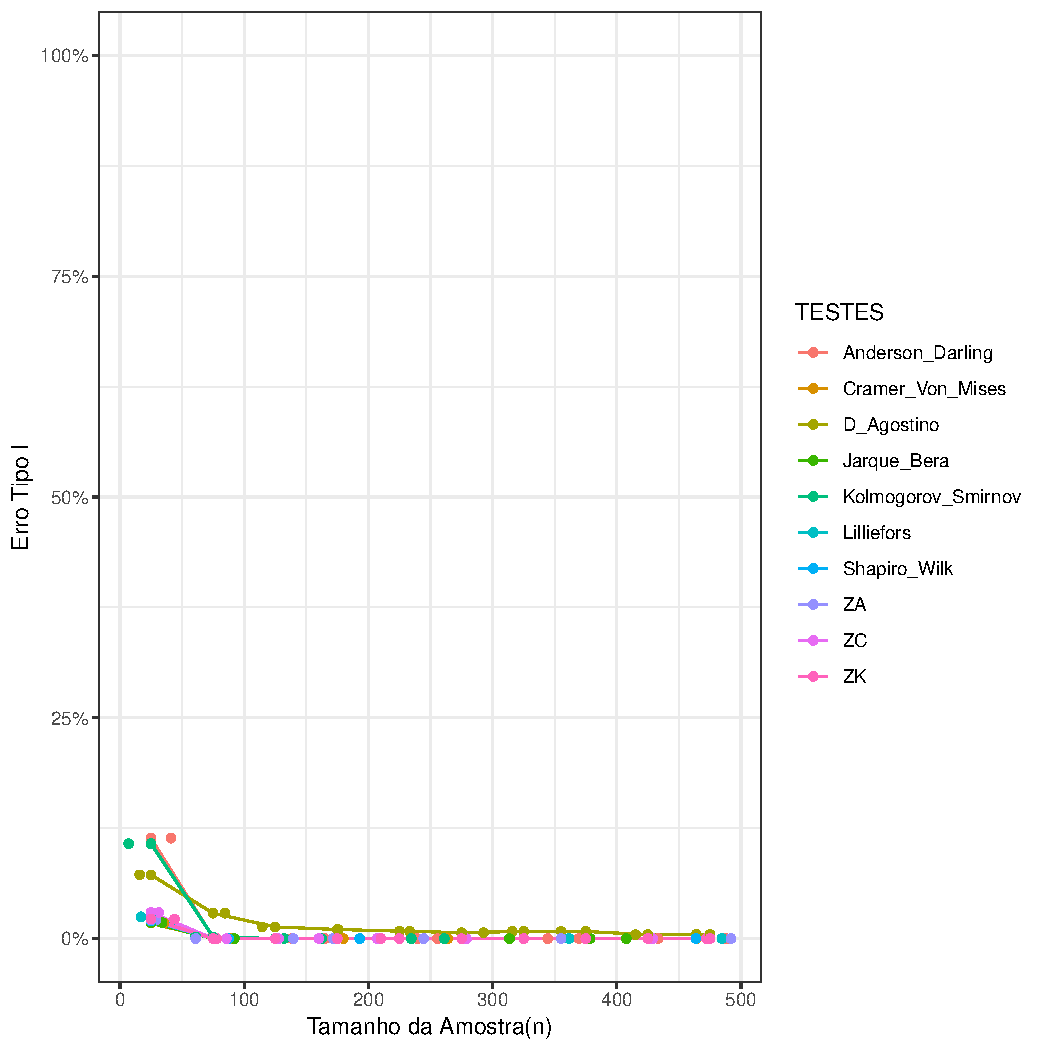
\includegraphics[width=0.95\textwidth]{Distribuição Cauchy/Erro Tipo I/erro_tipo_I_cauchy_500.pdf}
        \caption{Tamanho amostral \(n = 500\)}
        \label{fig:cauchy_500}
    \end{subfigure}
    \hfill
    \begin{subfigure}[b]{0.45\textwidth}
        \centering
        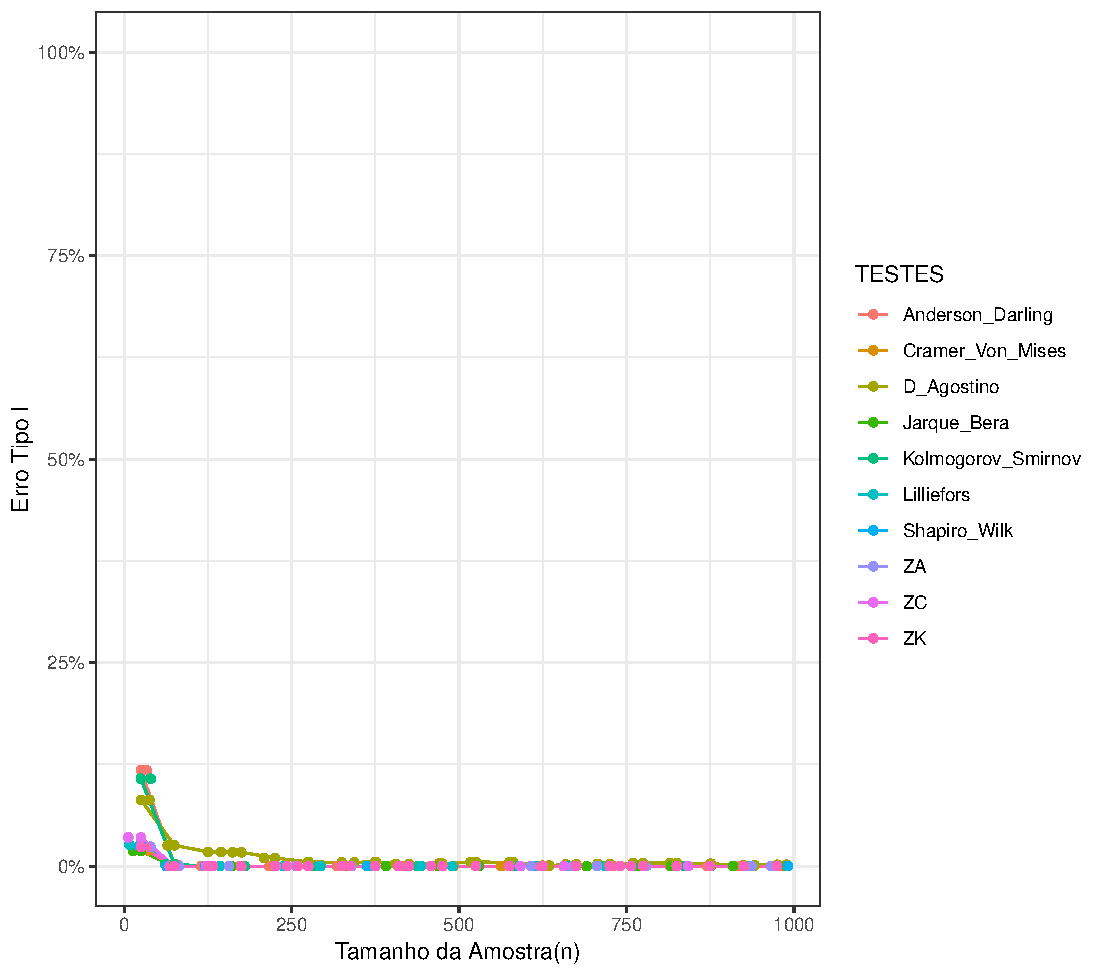
\includegraphics[width=0.95\textwidth]{Distribuição Cauchy/Erro Tipo I/erro_tipo_I_cauchy_1000.pdf}
        \caption{Tamanho amostral \(n = 1000\)}
        \label{fig:cauchy_1000}
    \end{subfigure}
\end{figure}

%%%%%%%%%% Poder do Teste -> Distribuição Cauchy %%%%%%%%%%
\begin{figure}[H]
    \centering
    \caption{Comparação do Poder do Teste dos testes AD, CM, DG, LL, JB, KS, ZA, ZC e ZK em função do tamanho amostral para a \textbf{Distribuição} \(\textbf{Cauchy}(0, 1)\).}
    \label{fig:poder_teste_dist_cauchy}
    
    % Primeira linha
    \begin{subfigure}[b]{0.45\textwidth}
        \centering
        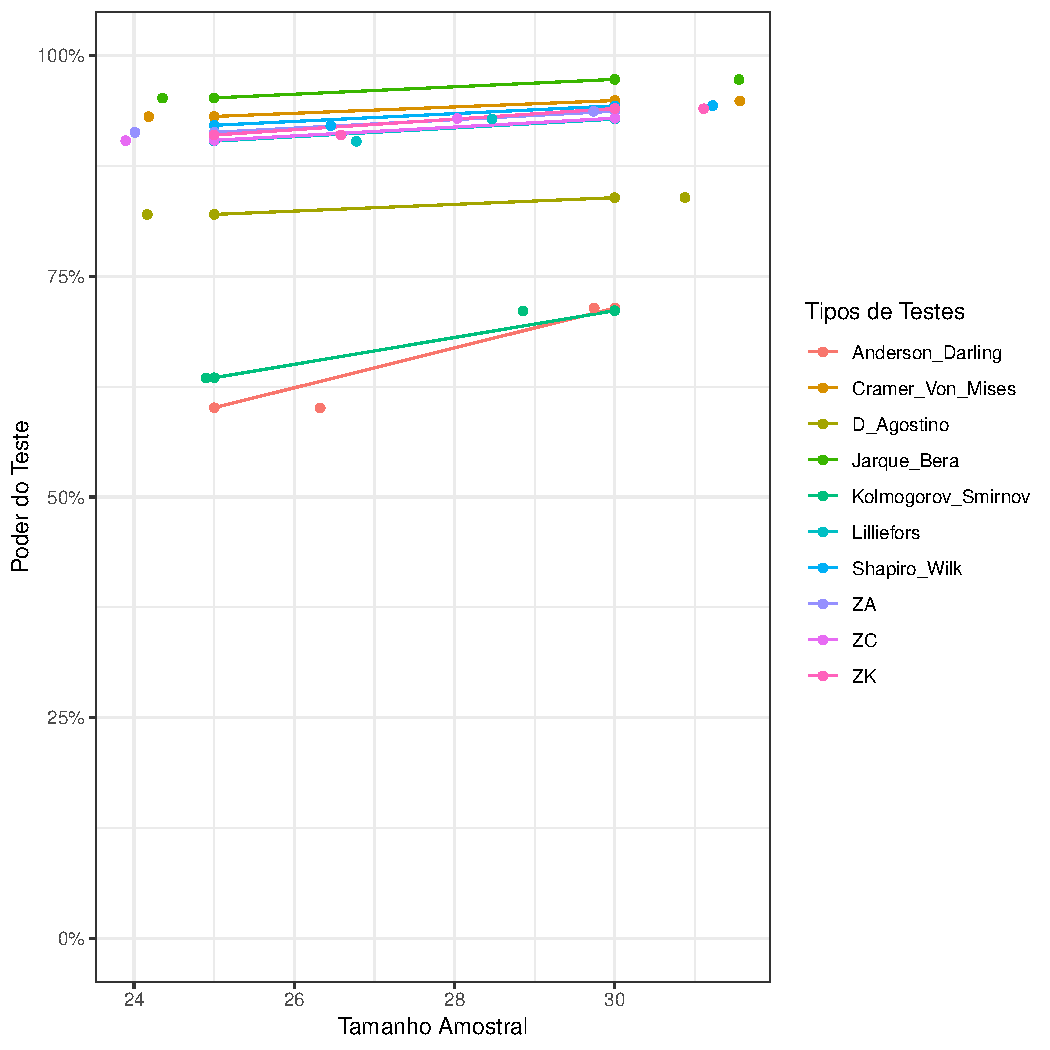
\includegraphics[width=0.95\textwidth]{Distribuição Cauchy/Poder do Teste/poder_teste_cauchy_30.pdf}
        \caption{Tamanho amostral \(n = 30\)}
        \label{fig:cauchy_poder_30}
    \end{subfigure}
    \hfill
    \begin{subfigure}[b]{0.45\textwidth}
        \centering
        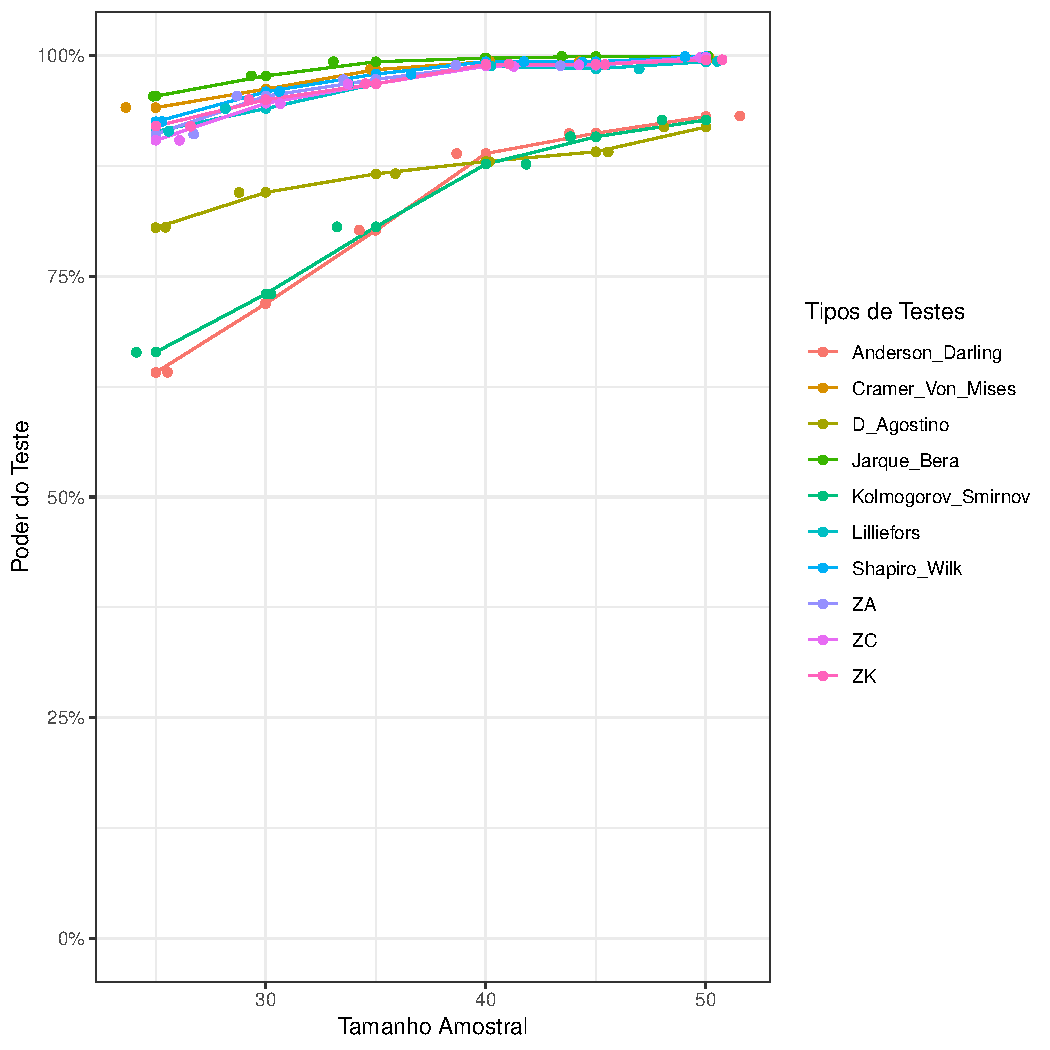
\includegraphics[width=0.95\textwidth]{Distribuição Cauchy/Poder do Teste/poder_teste_cauchy_50.pdf}
        \caption{Tamanho amostral \(n = 50\)}
        \label{fig:cauchy_poder_50}
    \end{subfigure}
    
    % Segunda linha
    \vspace{0.5cm} % Espaçamento entre linhas
    \begin{subfigure}[b]{0.45\textwidth}
        \centering
        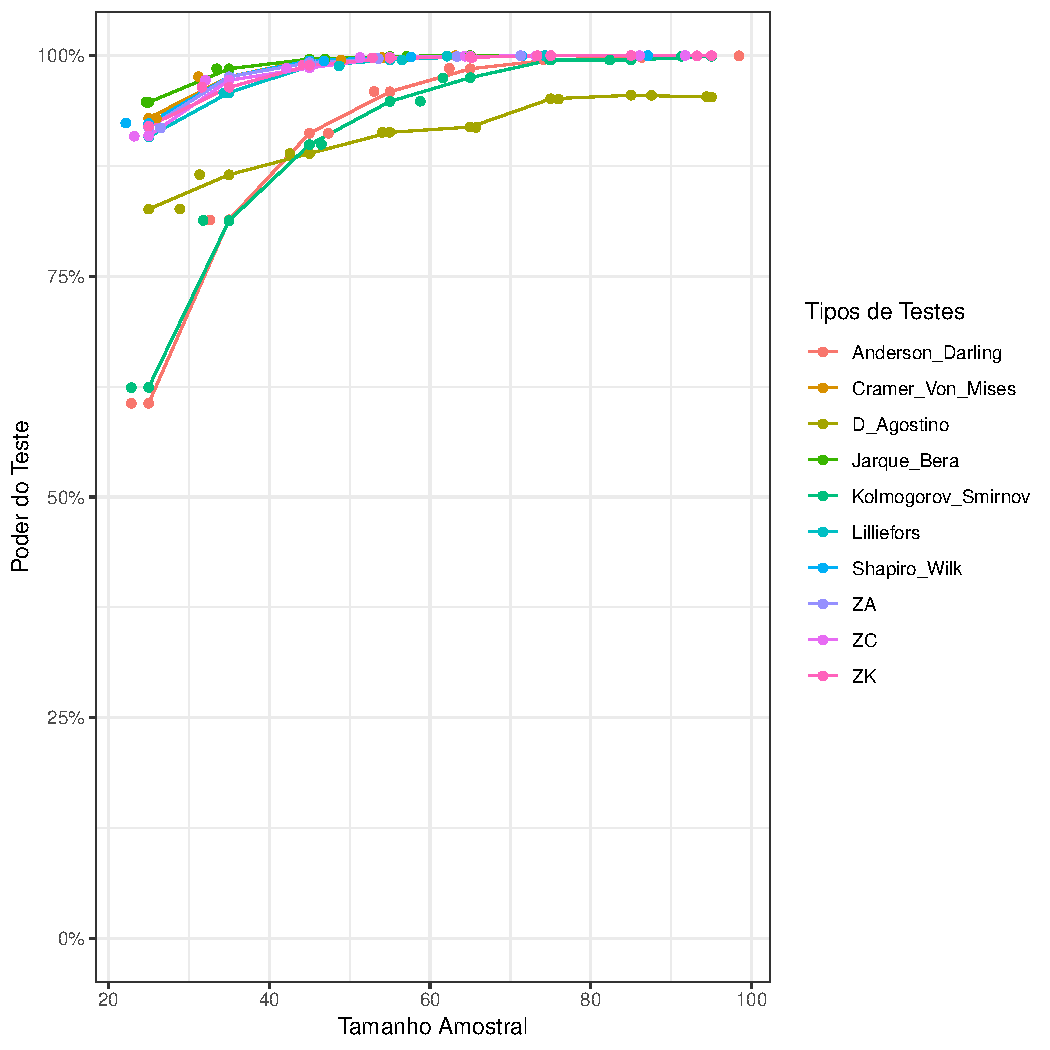
\includegraphics[width=0.95\textwidth]{Distribuição Cauchy/Poder do Teste/poder_teste_cauchy_100.pdf}
        \caption{Tamanho amostral \(n = 100\)}
        \label{fig:cauchy_poder_100}
    \end{subfigure}
    \hfill
    \begin{subfigure}[b]{0.45\textwidth}
        \centering
        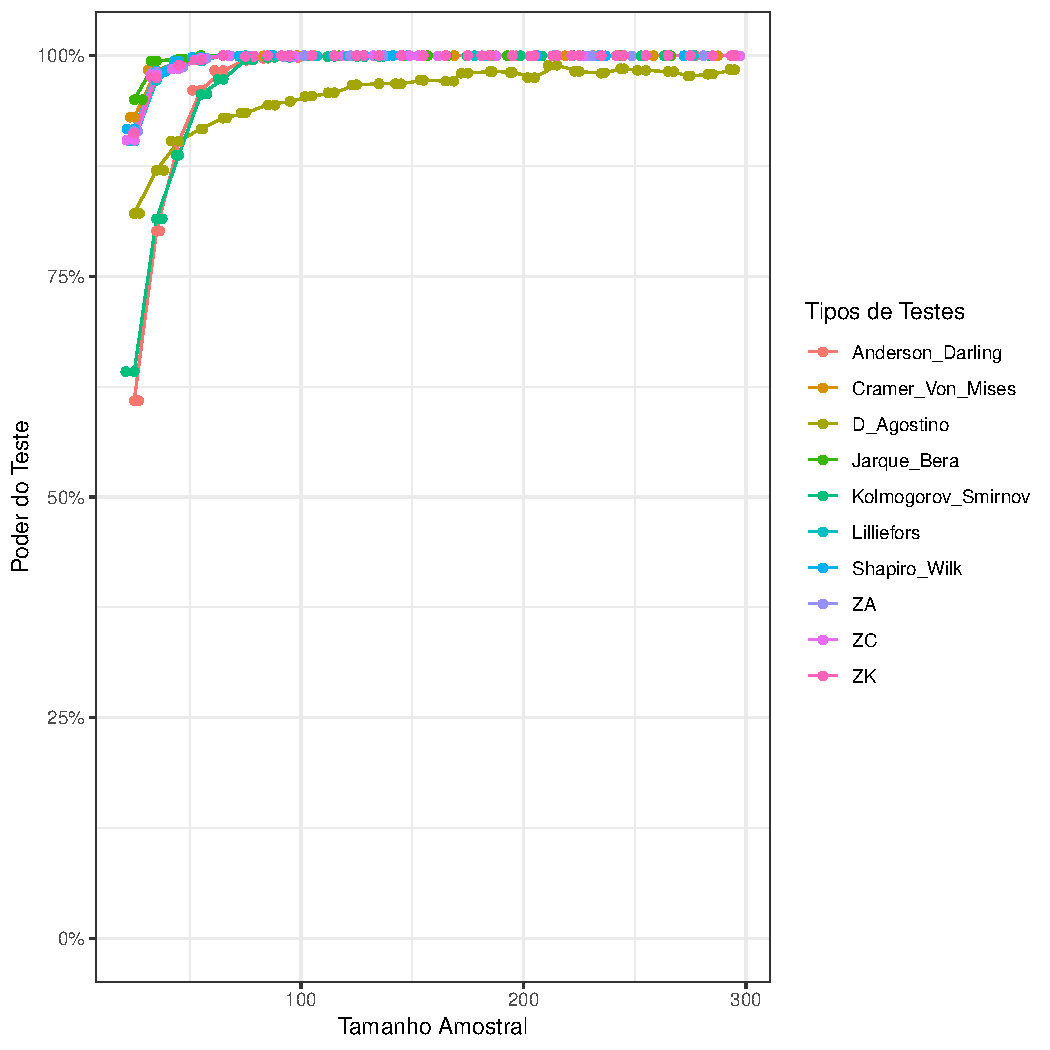
\includegraphics[width=0.95\textwidth]{Distribuição Cauchy/Poder do Teste/poder_teste_cauchy_300.pdf}
        \caption{Tamanho amostral \(n = 300\)}
        \label{fig:cauchy_poder_300}
    \end{subfigure}
    
    % Terceira linha
    \vspace{0.5cm} % Espaçamento entre linhas
    \begin{subfigure}[b]{0.45\textwidth}
        \centering
        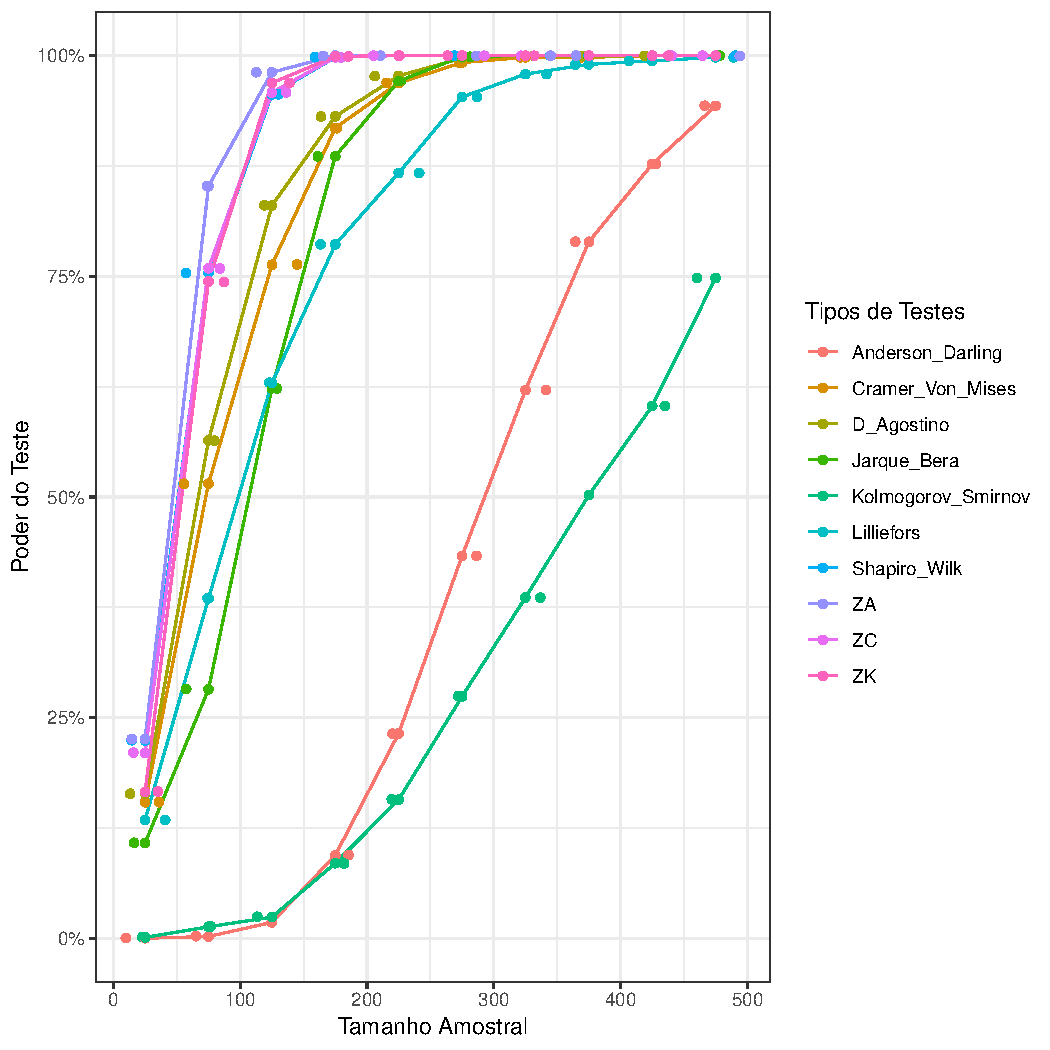
\includegraphics[width=0.95\textwidth]{Distribuição Beta/Poder do Teste/poder_teste_beta_500.pdf}
        \caption{Tamanho amostral \(n = 500\)}
        \label{fig:cauchy_poder_500}
    \end{subfigure}
    \hfill
    \begin{subfigure}[b]{0.45\textwidth}
        \centering
        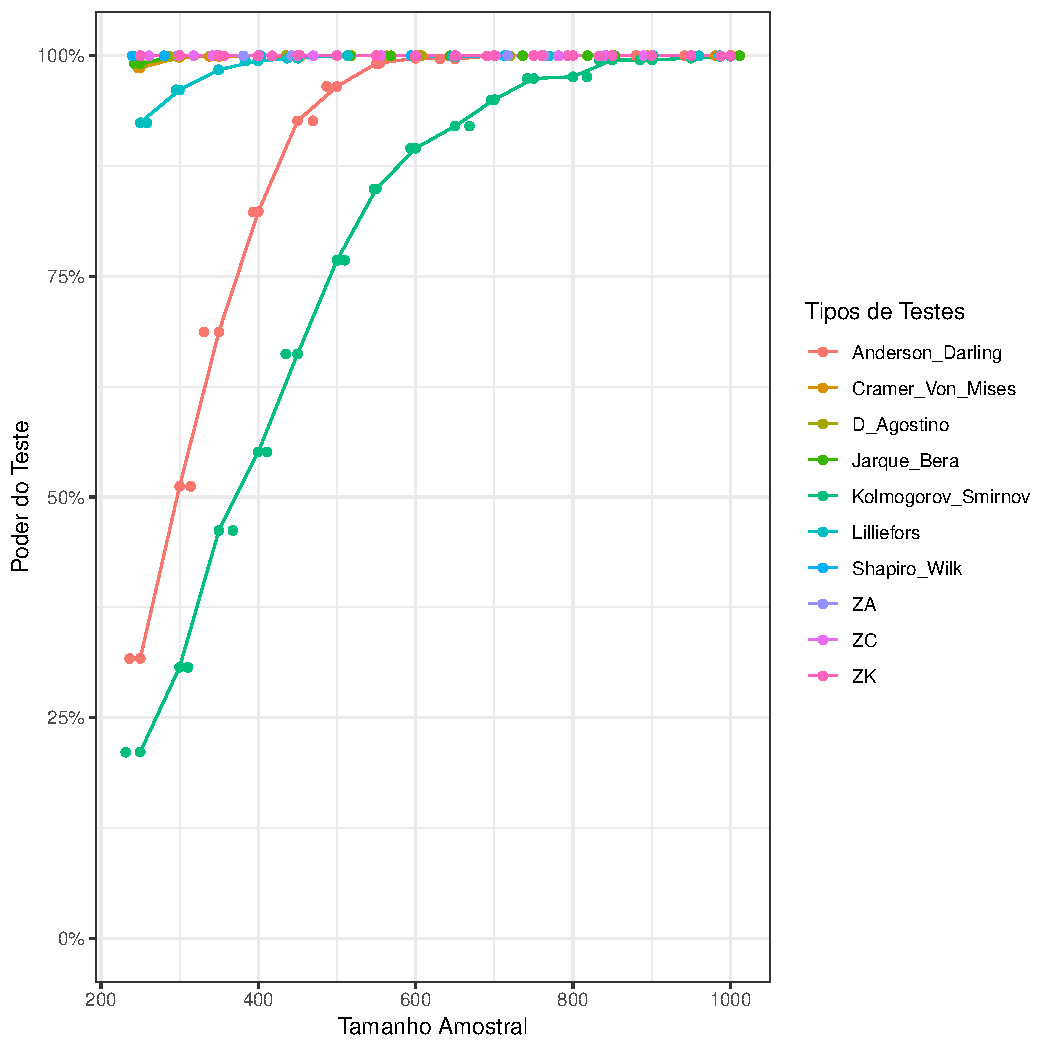
\includegraphics[width=0.95\textwidth]{Distribuição Beta/Poder do Teste/poder_teste_beta_1000.pdf}
        \caption{Tamanho amostral \(n = 1000\)}
        \label{fig:cauchy_poder_1000}
    \end{subfigure}
\end{figure}

%%%%%%%%%%%%%%%%%%%%%%%%%%%%%%%%%%%%%%%%%%%%%%%%%%%%%%%%%%%%%%%%%%%%%%%%%%%%%%%%%%%%%%%%%%%%
Observa-se na Figura (\ref{fig:erro_tipo_I_dist_norm}), que ilustra as Taxas de Erro Tipo I em função do tamanho amostral, que três testes apresentam desempenho inferior ao esperado: \textit{Kolmogorov-Smirnov}, \textit{Anderson-Darling} e \textit{Jarque-Bera}. Esses testes exibem taxas de Erro Tipo I consideravelmente distantes de 50\%, o que seria o esperado para dados provenientes de uma distribuição normal em testes de normalidade.

\vspace{0.5cm}

Embora o teste \textit{Jarque-Bera} tenda a se aproximar desse valor à medida que o tamanho da amostra aumenta, os testes \textit{Kolmogorov-Smirnov} e \textit{Anderson-Darling} permanecem substancialmente afastados do desempenho ideal, mesmo em tamanhos amostrais maiores.

\vspace{0.5cm}

Por outro lado, os demais testes apresentaram resultados consistentes com o esperado, exibindo Taxas de Erro Tipo I próximas a 50\% e com variações mínimas ao redor desse valor.

\vspace{0.5cm}

Ao analisar a Figura (\ref{fig:poder_teste_dist_norm}), em conjunto com as informações fornecidas pela Figura (\ref{fig:erro_tipo_I_dist_norm}), fica evidente que os testes \textit{Kolmogorov-Smirnov} e \textit{Anderson-Darling} não são os mais apropriados para avaliar a normalidade dos dados.

\vspace{0.5cm}

Isso se deve ao fato de que o \textit{Poder do Teste} desses métodos permaneceu consistentemente inferior ao dos demais testes avaliados, independentemente do tamanho amostral. Assim, os resultados reforçam que os testes \textit{Kolmogorov-Smirnov} e \textit{Anderson-Darling} possuem uma capacidade limitada de detectar desvios da normalidade, sendo menos poderosos quando comparados aos outros métodos analisados.

\vspace{0.5cm}

A Figura (\ref{fig:erro_tipo_I_dist_beta}) apresenta as taxas de Erro Tipo I dos testes de normalidade aplicados à distribuição Beta, caracterizada por sua assimetria. Observa-se que, para pequenos tamanhos amostrais, as taxas de Erro Tipo I exibem uma tendência linear decrescente em função de $n$. À medida que o tamanho amostral aumenta, essa relação evolui gradualmente para um comportamento de decaimento exponencial.

\vspace{0.5cm}

Quando $n \to \infty$, as taxas de Erro Tipo I convergem para valores próximos de zero. Isso indica que, para amostras muito grandes, a probabilidade de rejeitar $H_{0}$ quando ela é verdadeira ($\alpha$) se torna extremamente baixa ou até nula. Esse comportamento evidencia uma limitação dos testes de normalidade na detecção de desvios em distribuições assimétricas à medida que o tamanho amostral cresce.

\vspace{0.5cm}

Entre os testes avaliados, destacam-se \textit{Kolmogorov-Smirnov} e \textit{Anderson-Darling}, que apresentaram uma probabilidade de rejeição de $H_{0}$ mais elevada do que os outros testes, mesmo quando $H_{0}$ é verdadeira. Esses testes mostram maior dificuldade em convergir para taxas de Erro Tipo I próximas de zero, o que os torna menos adequados para avaliar a normalidade em distribuições assimétricas.

\vspace{0.5cm}

Por outro lado, os testes propostos por Zhang (2002) se destacaram por apresentar as menores taxas de Erro Tipo I, além de convergir mais rapidamente para zero à medida que o tamanho amostral aumenta. Esses resultados reforçam a superioridade dos métodos de Zhang na avaliação de normalidade em cenários envolvendo distribuições assimétricas.

\vspace{0.5cm}

A Figura (\ref{fig:poder_teste_dist_beta}) apresenta o Poder do Teste em função do tamanho amostral ($n$) para os testes de normalidade aplicados à distribuição $Beta(2, 5)$.

\newpage

Conforme observado na Figura anterior (\ref{fig:erro_tipo_I_dist_beta}), as Taxas de Erro Tipo I exibem um decaimento exponencial em função de $n$. De forma inversa e análoga, a Figura (\ref{fig:poder_teste_dist_beta}) revela que o Poder do Teste inicialmente cresce de maneira linear e, gradualmente, assume um comportamento logarítmico à medida que o tamanho amostral aumenta. Isso implica que, com amostras maiores, o Poder do Teste converge para valores próximos a 100\%, ou até atinge 100\%, evidenciando a capacidade dos testes em detectar desvios de normalidade.

\vspace{0.5cm}

Os resultados também indicam claramente quais testes são mais poderosos e quais apresentam desempenho inferior. Mais uma vez, os testes propostos por Zhang (2002) destacaram-se como os mais poderosos, alcançando rapidamente o Poder de Teste próximo a 100\%. Em contraste, os testes de Kolmogorov-Smirnov e Anderson-Darling continuam a apresentar baixo poder e demoram mais, de forma considerável, para atingir a convergência total, reforçando suas limitações em contextos de assimetria.

\vspace{0.5cm}

A Figura (\ref{fig:erro_tipo_I_dist_cauchy}) evidencia que os testes \textit{Kolmogorov-Smirnov} e \textit{Anderson-Darling} apresentaram, mais uma vez, as maiores Taxas de Erro Tipo I para a distribuição em teste ($Cauchy(0, 1)$), seguidos pelo teste \textit{D'Agostino}. Em contraste, os demais testes exibiram taxas mais aceitáveis e com menor variação. Entre estes, o teste \textit{Jarque-Bera} destacou-se, ainda que com uma diferença sutil, como aquele com as menores Taxas de Erro Tipo I.

À medida que o tamanho amostral ($n$) aumentou, as diferenças entre o teste \textit{Jarque-Bera} e os outros testes tornaram-se cada vez mínima. Com o crescimento de $n$, todas as taxas de Erro Tipo I convergiram para valores próximos de zero. No entanto, os testes \textit{D'Agostino}, e especialmente \textit{Kolmogorov-Smirnov} e \textit{Anderson-Darling}, foram os mais lentos em atingir essa convergência, evidenciando suas limitações na análise de distribuições similares a $Cauchy(0, 1)$, ou, como visto, a própria  $Cauchy(0, 1)$.

\vspace{0.5cm}

A Figura (\ref{fig:poder_teste_dist_cauchy}) mostra o Poder do Teste em função do tamanho amostral para a distribuição $Cauchy(0, 1)$. Nota-se que os testes \textit{Kolmogorov-Smirnov} e \textit{Anderson-Darling} se mostraram como os testes menos poderosos, um pouco acima deles está o teste \textit{D'Agostino}. Os demais testes mostraram poucas diferenças entres si, com  do teste \textit{Jarque-Bera}, que por uma pequena diferença, se mostrou o teste mais poderoso para amostras de tamanho 30, 50, 100 e 300.

Assim como nas demais Figuras, conforme se aumentou o tamanho da amostra, o Poder do Teste tende a 100\%. Kolmogorov-Smirnov e Anderson-Darling são os testes que mais demoraram a maximizar o Poder do Teste, seguidos pelo teste D'Agostino nessa marca. Outro ponto importante é que, para amostras de tamanho  

\section{Considerações Finais}

Texto em aberto.


\begin{comment}

\section*{Referências}

\begin{flushleft}

\noindent ANDERSON, T. W.; DARLING, D. A. Asymptotic theory of certain goodness of fit criteria based on stochastic processes. {\it The Annals of Mathematical Statistics}, JSTOR, p. 193–212, 1952.\newline
    
\noindent DARLING, D. A. The Kolmogorov-Smirnov, Cramer-von Mises tests. {\it The Annals of Mathematical Statistics}, JSTOR, v. 28, n. 4, p. 823–838, 1957.\newline


\noindent Dallal, G.E. and Wilkinson, L. (1986): An analytic approximation to the distribution of Lilliefors’test for normality. The American Statistician, 40, 294–296.\newline


\noindent D'Agostino, Ralph B.; Pearson, E. S. (1973). "Tests for Departure from Normality. Empirical Results for the Distributions of b2 and b1. Biometrika. 60(3): 613–622
\newline
    
\noindent DUFOUR, J. - M. et al. Simulation-based finite sample normality tests in linear regressions. {\it The Econometrics Journal}, Wiley Online Library, v. 1, n. 1, p. 154–173, 1998.\newline

\noindent Glasserman, P. (2004). Monte Carlo Methods in Financial Engineering. Springer.
\newline
    
\noindent JARQUE, C. M.; BERA, A. K. Efficient tests for normality, homoscedasticity and serial independence of regression residuals. {\it Economics Letters}, Elsevier, v. 6, n. 3, p. 255–259, 1980.\newline

\noindent JIN ZHANG, 2002. "Powerful goodness‐of‐fit tests based on the likelihood ratio," Journal of the Royal Statistical Society Series B, Royal Statistical Society, vol. 64(2), pages 281-294, May.\newline

\noindent LILLIEFORS, H. W. On the Kolmogorov-Smirnov test for normality with mean and variance unknown. {\it Journal of the American Statistical Association}, Taylor \& Francis, v. 62, n. 318, p. 399–402, 1967.\newline

\noident Lopes, M. de M., Castelo Branco, V. T. F., & Soares, J. B. (2013). Utilização dos testes estatísticos de Kolmogorov-Smirnov e Shapiro-Wilk para verificação da normalidade para materiais de pavimentação. TRANSPORTES, 21(1), 59–66. \newline

\noindent MEYER, Paul, L. – Probabilidade: Aplicação à Estatística – Ed. Livro Técnico, 1987. \newline

\noindent Metropolis, N., & Ulam, S. (1949). The Monte Carlo Method. Journal of the American Statistical Association.\newline

\noindent OLIVEIRA, I.R.C.; FERREIRA, D.F. Multivariate extension of chi-squared univariate normality test. J. Stat. Comput. Simul.), London, v.80, n.5, p.513-526, 2010.\newline

\noindent R CORE TEAM (2024). {\it R: A language and environment for statistical computing}. R Foundation for Statistical Computing, Vienna, Austria. Disponível em: \url{http://www.R-project.org/}.\newline

\noindent Rubinstein, R. Y., & Kroese, D. P. (2016). Simulation and the Monte Carlo Method. Wiley.

\noindent SHAPIRO, S. S.; WILK, M. B. An analysis of variance test for normality (complete samples). {\it Biometrika}, JSTOR, v. 52, n. 3/4, p. 591–611, 1965.\newline

\noindent STEPHENS, M.A. (1974): EDF statistics for goodness of fit and some comparisons. Journal of the American Statistical Association, 69, 730–737.\newline
    
\noindent STEPHENS, M. A. The Anderson-Darling statistic. {\it Stanford University}, 1979.\newline

\noindent STEPHENS, M.A. (1986): Tests based on EDF statistics. In: D’Agostino, R.B. and Stephens, M.A., eds.: Goodness-of-Fit Techniques. Marcel Dekker, New York.\newline

\noindent THODE JUNIOR, HC. Testing for Normality, New York: M Decker, 2002, 154p.




\end{flushleft}
    
\end{comment}

{ \large
\bibliographystyle{apalike}
\bibliography{references}
}


\end{document}